\documentclass[preprint]{elsarticle}

\usepackage[utf8x]{inputenc}
\usepackage[T1]{fontenc}
\PrerenderUnicode{à}

%\usepackage[utf8]{inputenc}
%\usepackage[T1]{fontenc}
%%\PrerenderUnicode{à}
\usepackage{lineno}
\linenumbers


% Text organization
\usepackage{comment}
\usepackage{csquotes}
\usepackage{caption} % subfigures
\usepackage{subcaption}
\usepackage{enumitem}



\usepackage{amsmath}
\usepackage{amsfonts}
\usepackage{amssymb}
\usepackage{stmaryrd}
\usepackage{amsthm}
\SetSymbolFont{stmry}{bold}{U}{stmry}{m}{n}
\newtheorem{fact}{Fact}[section]
\theoremstyle{remark}
%\newdefinition{remark}{Remark}
%\newdefinition{example}{Example}
\newtheorem{remark}{Remark}
\newtheorem{example}{Example}
\usepackage{latexsym}
\usepackage{cmll}
\usepackage{xspace}

% graphics
\usepackage{mathdots}
\usepackage{nicematrix}
\setcounter{MaxMatrixCols}{20}
\usepackage{rotating}
\usepackage{tikz}
\usepackage{xcolor}
\definecolor{keywordcolor}{rgb}{0.7, 0.1, 0.1} % red
\definecolor{commentcolor}{rgb}{0.4, 0.4, 0.4} % grey
\definecolor{symbolcolor}{rgb}{0.0, 0.1, 0.6}  % blue
\definecolor{sortcolor}{rgb}{0.1, 0.5, 0.1}    % green
\definecolor{aawhite}{rgb}{0.97,0.97,0.97}
\definecolor{awhite}{rgb}{0.90,0.90,0.90}
\definecolor{lgreen}{rgb}{0.94,1.0,0.98}
\definecolor{dgreen}{rgb}{0.0,0.3,0.1}
\definecolor{sgreen}{rgb}{0.0,0.7,0.3}
\definecolor{lgreen}{rgb}{0.94,1.0,0.98}
\definecolor{bgreen}{rgb}{0.00,0.50,0.25}
\definecolor{dblue}{rgb}{0.0,0.1,0.6}
\definecolor{lorange}{rgb}{1, .85, .60}
\definecolor{lblue}{rgb}{.80, .90, .95}
\definecolor{mixed}{rgb}{0.0,0.3,0.3}
\definecolor{dred}{rgb}{0.6,0.2,0.0}
\definecolor{sred}{rgb}{0.7,0.2,0.0}
\definecolor{ddred}{rgb}{0.3,0.1,0.0}
\definecolor{turq}{rgb}{0.28,0.82,0.80}
\definecolor{lyellow}{rgb}{1.00,0.97,0.94}
\definecolor{mygreen}{rgb}{0,0.6,0}
\definecolor{mygray}{rgb}{0.5,0.5,0.5}
\definecolor{mymauve}{rgb}{0.58,0,0.82}
\definecolor{codegreen}{rgb}{0,0.6,0}
\definecolor{codegray}{rgb}{0.5,0.5,0.5}
\definecolor{codepurple}{rgb}{0.58,0,0.82}
\definecolor{backcolour}{rgb}{0.96,0.96,0.96}
%%%%% Supplies \sout to suggest text erasure, together with comments in some colored text
\usepackage[normalem]{ulem}

\usepackage{graphicx}

\usepackage{hyperref}
\hypersetup{
    colorlinks=true,
    linkcolor=sred,
    filecolor=magenta,
    urlcolor=cyan,
    citecolor=sgreen,
}


% code
\usepackage{listings}
\def\lstlanguagefiles{lstlean.tex}
\lstset{language=lean}
\usepackage{float}
\floatstyle{boxed}
\restylefloat{table}
\restylefloat{figure}

% macro
% \newcommand{\svdots}{\scriptscriptstyle \boldsymbol \vdots}
\newcommand{\perm}[1]{\scriptstyle \left\rmoustache #1 \right\rmoustache}
\newcommand{\bloch}[2]{\Block[draw=white,fill=lblue,line-width=.5mm,rounded-corners]{#1}{#2}} % https://en.wikipedia.org/wiki/Ernest_Bloch
\newcommand{\oloch}[2]{\Block[draw=white,fill=lorange,line-width=.5mm,rounded-corners]{#1}{#2}}
\newcommand{\conv}[1]{\overbracket[.5pt][1pt]{\underbracket[.5pt][1pt]{#1}}}

\newcommand{\NN}{\mathbb{N}}
\newcommand{\ZZ}{\mathbb{Z}}
\newcommand{\RR}{\mathbb{R}}

\newcommand{\floor}[1]{\left\lfloor #1 \right\rfloor}

\newcommand{\gl}{\text{\guillemotleft}}
\newcommand{\gr}{\text{\guillemotright}}


\newcommand{\ORPP}{\mathsf{ORPP}}
\newcommand{\rppf}{\mathsf{f}}
\newcommand{\rppg}{\mathsf{g}}
\newcommand{\rpph}{\mathsf{h}}
\newcommand{\rppId}{\mathsf{Id}}
\newcommand{\rppNe}{\mathsf{Ne}}
\newcommand{\rppSu}{\mathsf{Su}}
\newcommand{\rppPr}{\mathsf{Pr}}
\newcommand{\rppSw}{\mathsf{Sw}}
\newcommand{\rppCo}{\fatsemi}
\newcommand{\rppPa}{\Vert}
\newcommand{\rppIt}{\mathsf{It}}
\newcommand{\rppIta}{\mathsf{Ita}}
\newcommand{\rppItr}{\mathsf{Itr}}
\newcommand{\rppIf}{\mathsf{If}}
\newcommand{\rppinc}{\mathsf{inc}}
\newcommand{\rppdec}{\mathsf{dec}}
\newcommand{\rppmul}{\mathsf{mul}}
\newcommand{\rppsquare}{\mathsf{square}}
\newcommand{\rppless}{\mathsf{less}}
\newcommand{\rppcp}{\mathsf{cp}}
\newcommand{\rppcpi}{\mathsf{cp_{input}}}
\newcommand{\rpptr}{\mathsf{tr}}
\newcommand{\rppcu}{\mathsf{cu}}
\newcommand{\rppcui}{\mathsf{cu_{input}}}
\newcommand{\rppcustep}{\mathsf{cu_{step}}}
\newcommand{\rppdiv}{\mathsf{div}}
\newcommand{\rppdivstep}{\mathsf{div_{step}}}
\newcommand{\rppsqrt}{\mathsf{sqrt}}
\newcommand{\rppsqrtstep}{\mathsf{sqrt_{step}}}
\newcommand{\rpprewire}[1]{\lfloor #1 \rceil}
\newcommand{\rppmkpair}{\mathsf{mkpair}}
\newcommand{\rppmkpairi}{\mathsf{mkpair_{input}}}
\newcommand{\rppunpair}{\mathsf{unpair}}
\newcommand{\rppunpairi}{\mathsf{unpair_{input}}}
\newcommand{\rppunpairifwd}{\mathsf{unpair_{input, \rightarrow}}}
\newcommand{\rppprecstep}{\mathsf{prec_{step}}}
\newcommand{\rppprecfwd}{\mathsf{prec_{\rightarrow}}}
\newcommand{\rppprec}{\mathsf{prec}}
\newcommand{\rppconvert}{\mathsf{convert}}
\newcommand{\rppNu}{\mathsf{Nu}}
\newcommand{\rppZe}{\mathsf{Ze}}
\newcommand{\rppEz}{\mathsf{Ez}}
\newcommand{\rppbin}{\mathsf{bin}}


\newcommand{\prZero}{\mathtt{0}}
\newcommand{\prSucc}{\mathtt{S}}
\newcommand{\prPred}{\mathtt{P}}
\newcommand{\prProj}[2]{\mathtt{P}^{#1}_{#2}} % P^n_i
\newcommand{\prCom}[1]{\circ{[#1]}} % composition
\newcommand{\prPrec}{\mathtt{R}}
\newcommand{\pradd}{\mathtt{ADD}}
\newcommand{\prack}{\mathtt{ACK}}

% Macros
\newcommand{\RPP}{\textsf{RPP}\xspace}
\newcommand{\UPRF}{\textsf{UPRF}\xspace}
\newcommand{\PRF}{\textsf{PRF}\xspace}
\newcommand{\PR}{\textsf{PR}\xspace}
\newcommand{\CPP}{\textsf{C}\xspace}
\newcommand{\MATHLIB}{\textsf{mathlib}\xspace}
\newcommand{\LEAN}{\textsf{Lean}\xspace}
\newcommand{\COQ}{\textsf{Coq}\xspace}
\newcommand{\LEANFour}{\textsf{Lean 4}\xspace}
\newcommand{\RPRF}{\textsf{R}\PRF\xspace} % reversible primitive
\newcommand{\PISA}{\textsf{Pendulum ISA}\xspace}
\newcommand{\JMF}{\textsf{RI}\xspace} % Jacopini Mentrasti
\newcommand{\Janus}{\textsf{Janus}\xspace}
\newcommand{\Matita}{\textsf{Matita}\xspace}
\newcommand{\SRL}{\textsf{SRL}\xspace}
\newcommand{\Nat}{\mathbb{N}}
\newcommand{\Int}{\mathbb{Z}}
\newcommand{\yb}{\textcolor{blue}{y}}
\newcommand{\yr}{\textcolor{red}{y}}


\begin{document}

\begin{frontmatter}

%\title{A formal certification that Reversible Primitive Permutations are Primitive-recursive complete}
% \title{Certifying algorithms and relevant properties of Reversible Primitive Permutations with \LEAN}
\title{Certifying expressive power and algorithms\\  of Reversible Primitive Permutations with \LEAN}

%\author{Giacomo Maletto\inst{1} \and
%	    Luca Roversi\inst{2}\orcidID{0000-0002-1871-6109}}

\author[1]{Giacomo Maletto}
\ead{giacomo.maletto@edu.unito.it}

\author[2]{Luca Roversi}
\ead{luca.roversi@unito.it}

\affiliation[1]{
    organization={Università degli Studi di Torino, Dipartimento di Matematica},
    country={Italy}
}

\affiliation[2]{
    organization={Università degli Studi di Torino, Dipartimento di Informatica},
    country={Italy}
}

\begin{abstract}
Reversible primitive permutations (\RPP) is a class of recursive functions that models reversible computation. We present a proof, which has been verified using the proof-assistant \LEAN, that demonstrates \RPP can encode every primitive recursive function (\PRF-completeness) and that each \RPP can be encoded as a primitive recursive function (\PRF-soundness). Our proof of \PRF-completeness is simpler and fixes some errors in the original proof, while also introducing a new, more primitive reversible iteration scheme for \RPP. By keeping the formalization and semi-automatic proofs simple, we are able to identify a single programming pattern that can generate a set of reversible algorithms within \RPP: Cantor pairing, integer division quotient/remainder, and truncated square root. The proof of \PRF-soundness is a novel contribution. Finally, \LEAN source code is available for experiments on reversible computation whose properties can be certified.
\end{abstract}

\begin{keyword}
    Reversible computation \sep Primitive recursion \sep Lean
\end{keyword}

\end{frontmatter}

%=====================
\section{Introduction}
\label{section:Introduction}
Studies focused on questions posed by Maxwell, regarding the solidity of the principles which Thermodynamics is based on, recognized the fundamental role that Reversible Computation can play to that purpose.

Reversible Computation is a significant area in Computer Science that encompasses various aspects such as reversible hardware design, unconventional computational models (such as quantum or bio-inspired ones), parallel computation and synchronization issues, debugging techniques, and transaction roll-back in database management systems.
The book \cite{perumalla2013chc} is a comprehensive introduction to the subject; the book \cite{DBLP:books/daglib/0025734}, focused on the low-level aspects of Reversible Computation, concerning the realization of reversible hardware, and
\cite{DBLP:series/eatcs/Morita17}, focused on how models of Reversible Computation like Reversible Turing Machines (RTM), and Reversible Cellular Automata (RCA) can be considered universal and how to prove that they enjoy such a property, are complementary to, and integrate \cite{perumalla2013chc}.

This work focuses on the \emph{functional model} \RPP \cite{DBLP:journals/tcs/PaoliniPR20} of Reversible Computation.
\RPP stands for (the class of) Reversible Primitive Permutations, which can be seen as a possible reversible counterpart of \PRF, the class of Primitive Recursive functions \cite{rogers1967theory}.
We recall that \RPP, in analogy with \PRF, is defined as the smallest class built on some given basic reversible functions, closed under suitable composition schemes.
The very functional nature of the elements in \RPP is at the base of reasonably accessible proofs of the following properties:
\begin{itemize}
\item \RPP is \PRF-complete \cite{DBLP:journals/tcs/PaoliniPR20}: for every function $ F \in \PRF $ with arity $ n \in \NN $, both $ m \in \NN $ and \lstinline|f| in \RPP exist such that \lstinline|f| encodes $ F $, i.e.
$ \mbox{\lstinline|f(|}z,\overline{x},\overline{y}\mbox{\lstinline|) = (|}z+F(\overline{x}),\overline{x},\overline{y}\mbox{\lstinline|)|}$, for every $ \overline{x}\in \NN^n $, whenever all the $m$ variables in $ \overline{y} $ are set to the value $ 0 $.
Both $ z $ and the tuple $ \overline{y} $ are \emph{ancillae}. They can be thought of as temporary storage for intermediate computations of the encoding.

\item \RPP can be extended to become Turing-complete \cite{Paolini2018NGC} by means of a minimization scheme analogous to the one that extends \PRF to the Turing-complete class of \emph{Partial} Recursive Functions.

\item According to \cite{MatosRC2020}, \RPP and the reversible programming language \SRL \cite{matos03tcs} are equivalent, so the fix-point problem is undecidable for \RPP as well \cite{2318_1734164MatosPaoliniRoversiTCSICTCS18}.
\end{itemize}

We think that this study provides additional support for the idea that using recursive computational models like \RPP to express Reversible Computation allows for the relatively easy certification of the correctness or other properties of \RPP algorithms through proof-assistants, potentially leading to the discovery of new algorithms.

We recall that a proof-assistant is an integrated environment to formalize data-types, to implement algorithms on them, to formalize specifications and prove that they hold, increasing algorithms dependability.

%%%%%%%%%%%%%%%%%%%%%%%%%%%%
\paragraph{Contributions}
We show how to express \RPP and its evaluation mechanism inside the proof-assistant \LEAN \cite{Lean3}. We can certify the correctness of every reversible function of \RPP with respect to a given specification which means certifying all the main results in \cite{DBLP:journals/tcs/PaoliniPR20}. In more detail:
\begin{itemize}
    \item We give a strong guarantee that \RPP is \PRF-complete in three macro steps. We exploit that in \LEAN \MATHLIB library, \PRF is proved equivalent to a class of recursive \emph{unary} functions called \lstinline|primrec|. We define a data-type \lstinline|rpp| in \LEAN to represent \RPP. Then, we certify that, for any function \lstinline|f:primrec|, i.e. any unary \lstinline|f| with type \lstinline|primrec| in \LEAN, a function exists with type \lstinline|rpp| that encodes \lstinline|f:primrec|. Apart from fixing some bugs, our proof is fully detailed as compared to \cite{DBLP:journals/tcs/PaoliniPR20}. Moreover it is conceptually and technically simpler.

    \item We also give a strong guarantee that \RPP is \PRF-sound (that is, each \RPP is expressible as \PRF) thus completing the work in \cite{MalettoR22}, by proving that the two classes of functions have the same expressivity. Again, for the proof of this fact we exploit the definitions and theorems in \MATHLIB concerning primitive recursive functions.

    \item Concerning simplification, it follows from how the elements in \lstinline|primrec| work. It is characterized by the following aspects:
    \begin{itemize}
        \item we define a \emph{new} finite reversible iteration scheme subsuming the reversible iteration schemes in \RPP, and \SRL, but which is more primitive;

        \item we identify an algorithmic pattern which uniquely associates elements of
        $ \mathbb{N}^2$, and $ \mathbb{N}$ by counting steps in specific paths.
        The pattern becomes a reversible element in \lstinline|rpp| once fixed the parameter it depends on. Slightly different parameter instances generate reversible algorithms whose behavior we can certify in \LEAN. They are truncated Square Root, Quotient/Reminder of integer division, and Cantor Pairing \cite{Cantor1878,DBLP:journals/corr/Szudzik17}.
        The original proof in \cite{DBLP:journals/tcs/PaoliniPR20} that \RPP is \PRF-complete relies on Cantor Pairing, used as a stack to keep the representation of a \PRF function as element of \RPP reversible.
        Our proof in \LEAN replaces Cantor Pairing with a reversible representation of functions \lstinline|mkpair|/\lstinline|unpair| that \MATHLIB supplies as isomorphism $ \mathbb{N}\times\mathbb{N} \simeq \mathbb{N} $. The truncated Square Root is the basic ingredient to obtain reversible \lstinline|mkpair|/\lstinline|unpair|.
    \end{itemize}
\end{itemize}

%---------------------
\paragraph{Related work}
Concerning the formalization in a proof-assistant of the semantics, and its properties, of a formalism for Reversible Computation, we are aware of \cite{paoliniTYPES2015}. By means of the proof-assistant \Matita \cite{Asperti2007}, it certifies that a denotational semantics for the imperative reversible programming language \Janus \cite[Section 8.3.3]{perumalla2013chc} is fully abstract with respect to the operational semantics.

Concerning \emph{functional models} of Reversible Computation, we are aware of \cite{jacopini89tcs} which introduces the class of reversible functions \JMF, which is as expressive as the \emph{Partial} Recursive Functions. So, \JMF is stronger than \RPP; however we see \JMF as less abstract than \RPP for two reasons: (i) the primitive functions of \JMF depend on a given specific binary representation of natural numbers; (ii) unlike \RPP, which we can see as \PRF in a reversible setting, it is not evident to us that \JMF can be considered the natural extension of a total class analogous to \RPP.

Finally, this work, starting from relevant parts of the BSc Thesis \cite{MalettoBSc2021}, which comes with a \LEAN project \cite{MalettoRPPLEAN2021} that certifies both properties and algorithms of \RPP, strictly extends \cite{MalettoR22} with the proof that \RPP is \PRF-sound.

%---------------------
\paragraph{Contents}
Section~\ref{section:Reversible Primitive Permutations} recalls the class \RPP by commenting on the main design aspects that characterize its definition inside \LEAN.
Section~\ref{section:RPP algorithms} defines and proves correct new reversible algorithms central to the proof.
Section~\ref{section:The UPRF-completeness of RPP} recalls the main aspects of \lstinline|primrec|, and illustrates the key steps to port the original \PRF-completeness proof of \RPP to \LEAN.
Section~\ref{section:Each RPP is PRF} shows how we used the constructs present in the \MATHLIB library to prove the \PRF-soundness of \RPP.
Section~\ref{section:Conclusion and developments} is about possible developments.

%=====================
\section{Reversible Primitive Permutations (\RPP) }
\label{section:Reversible Primitive Permutations}

\begin{figure}
    \centering
        \begin{lstlisting}[basicstyle=\small]
        inductive rpp : Type
        -- Base functions
        | Id (n : ℕ) : rpp -- Identity
        | Ne : rpp         -- Sign-change
        | Su : rpp         -- Successor
        | Pr : rpp         -- Predecessor
        | Sw : rpp         -- Transposition or Swap
        -- Inductively defined functions
        | Co (f g : rpp) : rpp   -- Series composition
        | Pa (f g : rpp) : rpp   -- Parallel composition
        | It (f : rpp) : rpp     -- Finite iteration
        | If (f g h : rpp) : rpp -- Selection
        infix `‖`  : 55 := Pa -- Notation for the Parallel composition
        infix `;;` : 50 := Co -- Notation for the Series composition
        \end{lstlisting}
    \caption{The class \RPP as a data-type \lstinline|rpp| in \LEAN.}
    \label{fig:RPP-LEAN}
\end{figure}

We use the data-type \lstinline|rpp| in Figure~\ref{fig:RPP-LEAN}, as defined in \LEAN, to recall from \cite{DBLP:journals/tcs/PaoliniPR20} that the class \RPP is the smallest class of functions
that contains five base functions, named as in Figure~\ref{fig:RPP-LEAN}, and all the functions that we can generate by the composition schemes whose name is next to the corresponding clause in Figure~\ref{fig:RPP-LEAN}. For ease of use and readability the last two lines in Figure~\ref{fig:RPP-LEAN} introduce infix notations for series and parallel composition.


\begin{example}[A term of type \texttt{rpp}]
\label{example:A first legal term of type RPP}
In \lstinline|rpp| we can write \lstinline|(Id 1‖Sw);;(It Su)‖(Id 1);;(Id 1‖If Su (Id 1) Pr)| which we also represent as a diagram:
\scalebox{}{.85}{
\[
\begin{NiceMatrix}
x&\bloch{1-1}{\mbox{\lstinline|Id 1|}}&x&\bloch{2-1}{\mbox{\lstinline|It  Su|}}&x&\bloch{1-1}{\mbox{\lstinline|Id 1|}}&x
\\
y&\bloch{2-1}{\mbox{\lstinline|Sw|}}&z& &z+x&\bloch{2-1}{\mbox{\lstinline|If Su (Id 1) Pr|}}&z+x
\\
z&&y&\bloch{1-1}{\mbox{\lstinline|Id 1|}}&y&& w
\end{NiceMatrix}
\enspace ,
\]}
where:
$$ \begin{aligned}
    w & = \begin{cases}
        y+1 & \textrm{if}\ z+x>0 \\
        y & \textrm{if}\ z+x=0 \\
        y-1 & \textrm{if}\ z+x<0
    \end{cases}
\enspace .
\end{aligned} $$
The inputs are the names to the left-hand side of the blocks; the outputs are to their right-hand side.
The term here above is a series composition of three parallel compositions.
The first one composes a unary identity \lstinline|Id 1|, which leaves its unique input untouched, and \lstinline|Sw|, which swaps its two arguments. Then, the $ x $-times iteration of the successor \lstinline|Su|, i.e. \lstinline|It Su|, is in parallel with \lstinline|Id 1|: that is why one of the outputs of \lstinline|It Su| is $ z + x $. Finally, \lstinline|If Su (Id 1) Pr| selects which among \lstinline|Su|, \lstinline|Id 1|, and \lstinline|Pr| to apply to the argument $ y $, depending on the value of $ z+x $; in particular, \lstinline|Pr| is the function that computes the predecessor of the argument. Figure~\ref{fig:RPP-ev} will give the operational semantics which defines \lstinline|rpp| formally as a class of functions on $ \ZZ$, not on $ \NN $.
\qed
\end{example}

\begin{remark}[``Weak weakening'' of algorithms in \texttt{rpp}]
\label{remark:Weakening algorithms of RPP}
%We can certify that \lstinline|(f‖(Id m)) X = f X|, but not
%\lstinline|((Id m)‖f) X = f X|, for any $ \lstinline|X| $.
We typically drop \lstinline|Id m| if it is the last function of a parallel composition. For example, term and diagram in \textit{Example}~\ref{example:A first legal term of type RPP} become \lstinline|(Id 1‖Sw);;(It Su);;(Id 1‖If Su (Id 1) Pr)| and:
\[ \begin{NiceMatrix}
        x&\bloch{1-1}{\mbox{\lstinline|Id 1|}}&x&\bloch{2-1}{\mbox{\lstinline|It  Su|}}&x&\bloch{1-1}{\mbox{\lstinline|Id 1|}}&x
        \\
        y&\bloch{2-1}{\mbox{\lstinline|Sw|}}&z& &z+x&\bloch{2-1}{\mbox{\lstinline|If Su (Id 1) Pr|}}&z+x
        \\
        z&&y&&y&& w
    \end{NiceMatrix}
    \enspace ,
\]
where:
$$
\begin{aligned}
    w & = \begin{cases}
        y+1 & \textrm{if}\ z+x>0 \\
        y & \textrm{if}\ z+x=0 \\
        y-1 & \textrm{if}\ z+x<0
    \end{cases}
    \enspace .
\end{aligned}
$$
\textit{Remark}~\ref{remark:We keep the definition of ev simple} explains why.
\qed
\end{remark}

\begin{figure}
\centering
\begin{lstlisting}[basicstyle=\small]
      def arity : rpp → ℕ
        | (Id n)     := n
        | Ne         := 1
        | Su         := 1
        | Pr         := 1
        | Sw         := 2
        | (f ‖ g)    := f.arity + g.arity
        | (f ;; g)   := max f.arity g.arity
        | (It f)     := 1 + f.arity -- "It f" has an extra argument compared to "f"
        | (If f g h) := 1 + max (max f.arity g.arity) h.arity
\end{lstlisting}
\caption{Arity of every \lstinline|f: rpp|.}
\label{fig:RPP-arity}
\end{figure}
\noindent
The function in Figure~\ref{fig:RPP-arity} computes the arity of any \lstinline|f:rpp| from the structure of \lstinline|f|, once fixed the arities of the base functions; \lstinline|f.arity| is \LEAN dialect for the more typical notation ``\lstinline|arity(f)|''.

\begin{figure}
    \begin{subfigure}{.5\textwidth}
        \centering
        $\begin{NiceMatrix}
            x_0&\bloch{1-1}{\mbox{\lstinline|Id 1|}}&x_0
            \\
            &\vdots&
            \\
            x_{n-1}&\bloch{1-1}{\mbox{\lstinline|Id 1|}}&x_{n-1}
        \end{NiceMatrix}$
        \caption{\lstinline|n| unary identities of \RPP in parallel.}
        \label{fig:Id 1 || .. || Id 1}
    \end{subfigure}
    \hfill
    \begin{subfigure}{.45\textwidth}
        \centering
        $ \begin{NiceMatrix}
            x_0&\bloch{3-1}{\mbox{\lstinline|Id n|}}&x_0
            \\
            \vdots&&\vdots
            \\
            x_{n-1}&&x_{n-1}
        \end{NiceMatrix} $
        \caption{Single \lstinline|n|-ary identity \lstinline|rpp|.}
        \label{fig:Id n}
    \end{subfigure}
    \caption{\lstinline|n|-ary identities are base functions of \lstinline|rpp|.}
    \label{fig:multiple-wires}
\end{figure}
\noindent
Figure~\ref{fig:multiple-wires} remarks that \lstinline|rpp| considers \lstinline|n|-ary identities \lstinline|Id n| as primitive; in \RPP the function \lstinline|Id n| is obtained by parallel composition of \lstinline|n| unary identities.

\begin{figure}
\begin{lstlisting}
    def inv : rpp → rpp
      | (Id n)     := Id n -- self-dual
      | Ne         := Ne   -- self-dual
      | Su         := Pr
      | Pr         := Su
      | Sw         := Sw   -- self-dual
      | (f ‖ g)    := inv f ‖ inv g
      | (f ;; g)   := inv g ;; inv f
      | (It f)     := It (inv f)
      | (If f g h) := If (inv f) (inv g) (inv h)
    notation f `⁻¹` := inv f
\end{lstlisting}
\caption{Inverse \lstinline|inv f| of every \lstinline|f:rpp|.}
\label{fig:RPP-inv}
\end{figure}

For any given \lstinline|f:rpp|, the function \lstinline|inv| in Figure~\ref{fig:RPP-inv} builds an element with type \lstinline|rpp|. The definition of \lstinline|inv| lets the successor \lstinline|Su| be inverse of the predecessor \lstinline|Pr| and lets every other base function be self-dual.
Moreover, the function \lstinline|inv|distributes over finite iteration \lstinline|It|, selection \lstinline|If|, and parallel composition \lstinline|‖|, while it requires to exchange the order of the arguments before distributing over the series composition \lstinline|;;|. The last line with \lstinline|notation| suggests that \lstinline|f⁻¹| is the inverse of \lstinline|f|; we shall prove this fact once given the operational semantics of \lstinline|rpp|.

\begin{figure}
\begin{lstlisting}[basicstyle=\small]
   def ev : rpp → list ℤ → list ℤ
   | (Id n)     X                    := X
   | Ne         (x :: X)             := -x :: X
   | Su         (x :: X)             := (x + 1) :: X
   | Pr         (x :: X)             := (x - 1) :: X
   | Sw         (x :: y :: X)        := y :: x :: X
   | (f ;; g)   X                    := ev g (ev f X)
   | (f ‖ g)    X                    := ev f (take f.arity X) ++ ev g (drop f.arity X)
   | (It f)     (x :: X)             := x :: ((ev f)^[↓x] X)
   | (If f g h) (0 :: X)             := 0 :: ev g X
   | (If f g h) (((n : ℕ) + 1) :: X) := (n + 1) :: ev f X
   | (If f g h) (-[1 + n] :: X)      := -[1 + n] :: ev h X
   | _          X                    := X
   notation `‹` f `›` := ev f
\end{lstlisting}
\caption{Operational semantics of elements in \lstinline|rpp|.}
\label{fig:RPP-ev}
\end{figure}

\subsection{Operational semantics of {\normalfont \lstinline|rpp|}}
The function \lstinline|ev| in Figure~\ref{fig:RPP-ev} interprets an element of \lstinline|rpp| as a function from a list of integers to a list of integers. Originally, in \cite{DBLP:journals/tcs/PaoliniPR20}, \RPP is a class of functions with type $ \ZZ^n \rightarrow \ZZ^n $. We use \lstinline|list ℤ| in place of tuples of \lstinline|ℤ| to exploit  \LEAN library \MATHLIB and save a large amount of formalization.

Let us give a look at the clauses in Figure~\ref{fig:RPP-ev}.

The function \lstinline|Id n| leaves the input list \lstinline|X| untouched.
\lstinline|Ne| ``negates'', i.e.\@ takes the opposite sign of, the head of the list, while \lstinline|Su| increments, and \lstinline|Pr| decrements it.
\lstinline|Sw| is the transposition, or swap, that exchanges the first two elements of its argument.
The series composition \lstinline|f;;g| first applies \lstinline|f| and then
\lstinline|g|.
The parallel composition \lstinline|f‖g| splits \lstinline|X| into two parts. The ``topmost'' one \lstinline|(take f.arity X)| has as many elements as the arity of \lstinline|f|; the ``lowermost'' one \lstinline|(drop f.arity X)| contains the part of \lstinline|X| that can supply the arguments to \lstinline|g|. Finally, it concatenates the two resulting lists by the append \lstinline|++|.

\vspace{\baselineskip}
\noindent
\emph{Finite iteration} \lstinline|It f| is new:
\begin{itemize}
    \item it iterates \lstinline|f| as many times as the value of the head \lstinline|x| of the argument, if \lstinline|x| contains a non negative value;
    \item otherwise it is the identity on the whole \lstinline|x::X|.
\end{itemize}
We denote this behavior by means of \lstinline|(ev f)^[↓x]|: the notation \lstinline|f^n| stands for the \MATHLIB function \lstinline|Nat.iterate|,
while \lstinline|↓x| is custom notation for the \MATHLIB function \lstinline|int.to_nat|.

\vspace{\baselineskip}
\noindent
The selection \lstinline|If f g h| chooses one among \lstinline|f|, \lstinline|g|, and \lstinline|h|, depending on the argument head \lstinline|x|: it is \lstinline|g| with \lstinline|x = 0|, it is \lstinline|f| with \lstinline|x > 0|, and \lstinline|h| with \lstinline|x < 0|.
The last line of Figure~\ref{fig:RPP-ev} sets a handy notation for \lstinline|ev|.

\begin{remark}[We want to keep the definition of \texttt{ev} simple]
\label{remark:We keep the definition of ev simple}

Based on our definition, using \LEAN, we show that:
\begin{lstlisting}
    theorem ev_split (f: rpp) (X: list ℤ):
    ‹f› X = (‹f› (take f.arity X)) ++ drop f.arity X
\end{lstlisting}
holds. It is one of the most complex properties to prove because it essentially says that we can apply any \lstinline|‹f›| to \emph{any} \lstinline|X| with at least as many elements as \lstinline|arity f|.

The proof is based on two observations.

First, if \lstinline|X.length >= f.arity|, i.e.\@ \lstinline|X| supplies enough arguments, then \lstinline|f| operates on the first elements of \lstinline|X| according to its arity. This justifies \textit{Remark}~\ref{remark:Weakening algorithms of RPP}.

Second, if \lstinline|X.length < f.arity| holds, i.e.\@ \lstinline|X| has not enough elements, then \lstinline|f X| has an unspecified behavior; this might sound odd, but it simplifies the certified proofs of must-have properties of \lstinline|rpp|.
\qed
\end{remark}

%======================
\subsection{The functions \texorpdfstring{\normalfont \lstinline|inv h|}{inv h} and \texorpdfstring{\normalfont \lstinline|h|}{h} are each other inverse}
Once defined \lstinline|inv| in Figure~\ref{fig:RPP-inv} and \lstinline|ev| in Figure~\ref{fig:RPP-ev} we can prove:
\begin{lstlisting}
    theorem inv_co_l (h : rpp) (X : list ℤ) : ‹h ;; h⁻¹› X = X
    theorem inv_co_r (h : rpp) (X : list ℤ) : ‹h⁻¹ ;; h› X = X
\end{lstlisting}
certifying that \lstinline|h| and \lstinline|h⁻¹| are each other inverse.
We start by focusing on the main details to prove \lstinline|theorem inv_co_l| in \LEAN. The proof proceeds by (structural) induction on \lstinline|h|, which generates 9 cases, one for each clause that defines \lstinline|rpp|. One can go through the majority of them smoothly.
Some comments about two of the more challenging cases follow.

\paragraph{Parallel composition} Let \lstinline|h| be some parallel composition, whose main constructor is \lstinline|Pa|. The step-wise proof of \lstinline|inv_co_l| is:
\begin{lstlisting}
‹f‖g;;(f‖g)⁻¹› X
    = ‹f‖g;;f⁻¹‖g⁻¹› X       -- by definition
(!) = ‹(f;;f⁻¹)‖(g;;g⁻¹)› X  -- lemma pa_co_pa, arity_inv below
    = ‹f;;f⁻¹›(take f.arity X) ++ ‹g;;g⁻¹›(drop f.arity X)
                             -- by definition
    = take f.arity X ++ drop f.arity X -- by ind. hyp.
    = X                      -- property of ++ (append),
\end{lstlisting}
where the equivalence \lstinline|(!)| holds because we can prove both:
\begin{lstlisting}
lemma pa_co_pa (f f' g g' : rpp) (X : list ℤ) :
 f.arity = f'.arity → ‹f‖g ;; f'‖g'› X = ‹(f;;f') ‖ (g;;g')› X ,
lemma arity_inv (f : rpp) : f⁻¹.arity = f.arity .
\end{lstlisting}
Proving \lstinline|lemma arity_inv|, i.e. that the arity of a function does not change if we invert it, assures that we can prove \lstinline|lemma pa_co_pa|, i.e.\@ that series and parallel compositions smoothly distribute reciprocally.

\paragraph{Iteration} Let \lstinline|h| be a finite iterator whose main constructor is \lstinline|It|.
The goal to prove is \lstinline|‹It f;;It f⁻¹› x::X = x::X| which reduces to \lstinline|‹f⁻¹›^[↓x] (‹f›^[↓x] X') = X'|, where, we recall, the notation \lstinline|‹f›^[↓x]| means ``\lstinline|‹f›| applied \lstinline|x| times, if \lstinline|x| is positive''. This can be restated as the proposition \lstinline|function.left_inverse g^[n] f^[n]|, where
\begin{lstlisting}
def left_inverse (g : β → α) (f : α → β) : Prop :=
    ∀ x, g (f x) = x
\end{lstlisting}
is defined in \MATHLIB. We can make use of theorem \lstinline{function.left_inverse.iterate}, also present in \MATHLIB, which states that if \lstinline{function.left_inverse g f} is true, then also \lstinline|function.left_inverse g^[n] f^[n]| is.

\vspace{\baselineskip}
To conclude, let us see how the proof of \lstinline|inv_co_r| works. It does not copy-cat the one of \lstinline|inv_co_l|, which would require a lot of repetition. It instead relies on proving:
\begin{lstlisting}
   lemma inv_involute (f : rpp) : (f⁻¹)⁻¹ = f ,
\end{lstlisting}
\noindent
which says that applying \lstinline|inv| twice is the identity, and on using \lstinline|inv_co_l|:
\begin{lstlisting}
    ‹f⁻¹ ;; f› X = X -- which, by inv_involute, is equivalent to
    ‹f⁻¹ ;; (f⁻¹)⁻¹› X = X -- which holds because it is an instance of (inv_co_l f⁻¹) .
\end{lstlisting}

\begin{remark}[On our simplifying choices on {\normalfont \lstinline|ev|}]
\label{remark:On our simplifying choices on ev}
A less general, but semantically more appropriate version of  \lstinline|inv_co_l| and \lstinline|inv_co_r| could be:
\begin{lstlisting}
    theorem inv_co_l (f : rpp) (X : list ℤ) :
                f.arity ≤ X.length → ‹f ;; f⁻¹› X = X
    theorem inv_co_r (f : rpp) (X : list ℤ) :
                f.arity ≤ X.length → ‹f⁻¹ ;; f› X = X
\end{lstlisting}
because, recalling \textit{Remark}~\ref{remark:We keep the definition of ev simple}, the application \lstinline|(f X)| makes sense when \lstinline|f.arity ≤ X.length|.
Fortunately, the way we defined \lstinline|rpp| allows us to state \lstinline|inv_co_l| or \lstinline|inv_co_r| in full generality
with no reference to \lstinline|f.arity ≤ X.length|.
\end{remark}

%======================
\subsection{Changes from the original definition}
The definition of \lstinline|rpp| in \LEAN is really very close to the original \RPP, but not identical. The goal is to simplify the overall task of formalization and certification. The brief list of changes follows.
\begin{itemize}
    \item As already outlined, \lstinline|It| and \lstinline|If| use the head of the input list to iterate or choose: taking the head of a list with pattern matching is obvious. In \cite{DBLP:journals/tcs/PaoliniPR20}, it is the last element in the input tuple that drives iteration and selection of \RPP.

    \item \lstinline|Id n|, for any \lstinline|n:ℕ|, is primitive in \lstinline|rpp| and derived in \RPP.
%    In some cases it is useful to have \lstinline|Id 0| available.

    \item Using \lstinline|list ℤ → list ℤ| as the domain of the function that interprets any given element \lstinline|f:rpp| avoids  letting the type of \lstinline|f:rpp| depend on the arity of \lstinline|f|. To know the arity of \lstinline|f| it is enough to invoke \lstinline|arity f|. Finally, we observe that getting rid of a dependent type like, say, \lstinline|rpp n|, allows us to escape situations in which we would need to compare equal but not definitionally equal types like \lstinline|rpp (n+1)| and \lstinline|rpp (1+n)|.

    \item The new finite iterator \lstinline|It f (x::t): list ℤ| \emph{subsumes} the finite iterators \lstinline|ItR| in \RPP, and \lstinline|for| in \SRL. This means that \lstinline|It| is more primitive, but equally expressive and simpler for \LEAN to prove that its definition is terminating.

    More specifically, we recall that:
    \begin{itemize}
        \item \lstinline|ItR f (x₀,x₁,...,xₙ₋₂,x)| simply evaluates to \lstinline|f(f(...f(x₀,x₁,...,xₙ₋₂)...))| with $ \mid\!\!\mbox{\lstinline|x|}\!\!\mid $ occurrences of \lstinline|f|;

        \item \lstinline|for(f) (x₀,x₁,...,xₙ₋₂,x)| is slightly more complex:
        \begin{enumerate}
            \item it evaluates to \lstinline|f(f(...f(x₀,x₁,...,xₙ₋₂)...))|, with \lstinline|x| occurrences of \lstinline|f|, if \lstinline|x > 0|;

            \item it evaluates to \lstinline|f⁻¹(f⁻¹(...f⁻¹(x₀,x₁,...,xₙ₋₂)...))|, with \lstinline|-x| occurrences of \lstinline|f⁻¹|, if \lstinline|x < 0|;

            \item it behaves like the identity if \lstinline|x = 0|.
        \end{enumerate}
    \end{itemize}

    We know how to define both \lstinline|ItR| and \lstinline|for| in terms of \lstinline|It|:
    \begin{align}
    \label{align:It ItR}
        \mbox{\lstinline|ItR f|}
        & =
        \mbox{\lstinline|(It f);;Ne;;(It f);;Ne|} \\
    \label{align:It for}
        \mbox{\lstinline|for(f)|}
        & =
        \mbox{\lstinline|(It f);;Ne;;(It f⁻¹);;Ne|}
        \enspace .
    \end{align}
    \begin{example}[How does \eqref{align:It ItR} work?]
    \label{example:How align:It ItR works}
    Whenever \lstinline|x > 0|, the leftmost \lstinline|It f| in \eqref{align:It ItR} iterates \lstinline|f|, while the rightmost one does nothing because \lstinline|Ne| in the middle negates \lstinline|x|.
    On the contrary, if \lstinline|x < 0|, the leftmost \lstinline|It f| does nothing and the iteration is performed by the rightmost iteration, because \lstinline|Ne| in the middle negates \lstinline|x|. In both cases, the last \lstinline|Ne| restores \lstinline|x| to its initial sign. But this is the behavior of \lstinline|ItR|, as we wanted.
    \qed
    \end{example}
\end{itemize}

%=====================
\section{\RPP algorithms central to our proofs}
\label{section:RPP algorithms}

\begin{figure}
\begin{subfigure}{.225\textwidth}
\centering
\scalebox{.8}
{$\begin{NiceMatrix}
    n & \bloch{2-1}{\mbox{\lstinline|It Su|}} & n     \\
    x &                      & x + n \\
 \end{NiceMatrix}$
}\caption{Increment \footnotemark }
\label{sfig:inc}
\end{subfigure}
\hfill
\begin{subfigure}{.225\textwidth}
\centering
\scalebox{.8}
{$ \begin{NiceMatrix}
    n & \bloch{2-1}{\mbox{\lstinline|It Pr|}} & n     \\
    x &                      & x - n \\
  \end{NiceMatrix} $
}
\caption{Decrement \lstinline|dec|}
\label{sfig:dec}
\end{subfigure}
\hfill
\begin{subfigure}{.325\textwidth}
\centering
\scalebox{.8}
{$ \begin{NiceMatrix}
    n & \bloch{3-1}{\mbox{\lstinline|It inc|}} & n             \\
    m &                     & m             \\
    x &                     & x + n \cdot m \\
  \end{NiceMatrix} $
}\caption{Multiplication \lstinline|mul|}
\label{sfig:mul}
\end{subfigure}
\\ \\ \\
\begin{subfigure}{.6\textwidth}
\centering
\scalebox{.8}
{$\begin{NiceMatrix}
n&\bloch{1-1}{\mbox{\lstinline|Id 1|}}
  &n
   &\bloch{2-1}{\mbox{\lstinline|inc|}}
    &n
     &\bloch{3-1}{\mbox{\lstinline|mul|}}
      &n
       &\bloch{2-1}{\mbox{\lstinline|dec|}}
        &n
         &\bloch{1-1}{\mbox{\lstinline|Id 1|}}
          &n\\
x&\bloch{2-1}{\mbox{\lstinline|Sw|}}&0&&n&&n&&0&\bloch{2-1}{\mbox{\lstinline|Sw|}}&x+n^2\\
0&&x&&x&&x+n^2&&x+n^2&& 0
\end{NiceMatrix}$
}
\caption{\lstinline|square|}
\label{fig:square}
\end{subfigure}
\hfill
\begin{subfigure}{.325\textwidth}
    \centering
\scalebox{.8}
{    $\begin{NiceMatrix}
        x_0 & \bloch{6-1}{\rpprewire{i_0, \ldots, i_n}} & x_{i_0} \\
      \cdot &                                & \vdots  \\
      \cdot &                                & x_{i_n} \\
      \cdot &                                & x_{j_1} \\
      \cdot &                                & \vdots  \\
        x_m &                                & x_{j_{m-n}}
    \end{NiceMatrix}$
}    \caption{Rewiring $ \rpprewire{i_0 \ldots i_n} $}
    \label{fig:rewiring}
\end{subfigure}
\caption{Some useful functions of \lstinline|rpp|}
\label{fig:standard functions}
\end{figure}
\footnotetext{Note that using our definition, the variable \lstinline|n| must be non-negative in order to have the shown behavior,
otherwise the function acts as the identity. This is why it's called {\it increment} and not {\it addition}.}

Figure~\ref{fig:standard functions} recalls definition, and behavior of some \lstinline|rpp| functions already introduced in \cite{DBLP:journals/tcs/PaoliniPR20}.

It is worth commenting on how the function \emph{rewiring} $ \rpprewire{i_0 \ldots i_n} $ works. Let $\{ i_0, \dots, i_n \} \subseteq \{ 0, \dots, m \}$ be a set of $n+1$ distinct indices between $0$ and $m$, and $\{ j_1, \dots, j_{m-n} \} = \{ 0, \dots, m \} \setminus \{ i_0, \dots, i_n \}$ which we assume such that $j_k < j_{k+1}$, for every $ 1 \leq k < m-n $.
By definition, $\rpprewire{i_0, \dots, i_n} (x_0, \dots, x_m) = (x_{i_0}, \dots, x_{i_n},$ $x_{j_1}, \dots, x_{j_{m-n}})$, i.e.\@ rewiring brings every input with index in $ \{ i_0, \dots,  i_n \} $ in front of all the inputs with index in $\{ j_1, \dots, j_{m-n} \}$, preserving the order.

\subsection{The algorithm scheme {\normalfont \texttt{step[\_]}}}
Figure~\ref{fig:function scheme step} identifies the \emph{new algorithm scheme} \lstinline|step[_]|. Depending on how we fill the hole \lstinline|[_]|, we get step functions that, once iterated, draw paths in $ \NN^2 $.
%The names $ a_0, \ldots, b_0, \ldots $ are just place holders, currently.

On top of the functions in Figures~\ref{fig:standard functions}, and~\ref{fig:function scheme step} we build Cantor Pairing/Un-pairing, Quotient/Reminder of integer division, and truncated Square Root. Suitable instances of \lstinline|step[_]| allow us to visit $ \NN^2 $ as in Figures~\ref{sfig:cantor as a path}, \ref{sfig:Quot./Rem.}, and~\ref{sfig:Square root}, respectively. The pairing function $\rppmkpair$, which behaves as in Figure~\ref{sfig:mkpair}, and which is an alternative to Cantor Pairing/Unpairing, has a more complex definition; it will be a necessary ingredient of our main proof.

\begin{figure}
    \centering
    \scalebox{.825}{
        $\begin{NiceMatrix}
            &\bloch{1-1}{\mbox{\lstinline|Id 1|}} & \bloch{3-1}{\rpprewire{2,0,1}} & \bloch{3-1}{\mbox{\lstinline|If(Su‖Pr)[_](Id 2)|}} & \bloch{2-1}{\mbox{\lstinline|Sw|}} & \bloch{2-1}{\mbox{\lstinline|If(Pr)(Id 1)(Id 1)|}} &\bloch{1-1}{\mbox{\lstinline|Id 1|}}\\
            &\bloch{2-1}{\mbox{\lstinline|If(Su)(Id 1)(Id 1)|}}&&     &&    & \bloch{2-1}{\mbox{\lstinline|Sw|}}\\
            &&&&&
        \end{NiceMatrix}$
       }
    \caption{Algorithm scheme \lstinline|step[_]|. The algorithm we can obtain from it depends on how we fill the hole \lstinline|[_]|.}
    \label{fig:function scheme step}
\end{figure}

\begin{figure}
\begin{subfigure}{.225\textwidth}
\centering
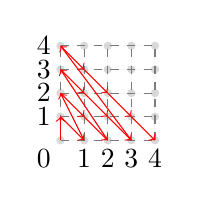
\begin{tikzpicture}[scale=0.3]
    % grid
    \draw[dashed,fill=gray,opacity=.5]  (0,0) grid (4,4);
    % labels
    \foreach \x in {1,...,4} { \node [anchor=north] at (\x,0) {\x}; }
    \foreach \y in {1,...,4} { \node [anchor=east] at (0,\y) {\y}; }
    \node [anchor=north east] at (0,0) {0};
    % vertices
    \foreach \x in {0,...,4} {
        \foreach \y in {0,...,4} {
            \node at (\x,\y) [circle,inner sep=0pt,minimum size=3pt,fill=gray,opacity=.3] {};
        }
    }
    % path
    \draw [->,red] (0,0) -- (0,1);
    \draw [->,red] (0,1) -- (1,0);
    \draw [->,red] (1,0) -- (0,2);
    \draw [->,red] (0,2) -- (1,1);
    \draw [->,red] (1,1) -- (2,0);
    \draw [->,red] (2,0) -- (0,3);
    \draw [->,red] (0,3) -- (1,2);
    \draw [->,red] (1,2) -- (2,1);
    \draw [->,red] (2,1) -- (3,0);
    \draw [->,red] (3,0) -- (0,4);
    \draw [->,red] (0,4) -- (1,3);
    \draw [->,red] (1,3) -- (2,2);
    \draw [->,red] (2,2) -- (3,1);
    \draw [->,red] (3,1) -- (4,0);
\end{tikzpicture}
\caption{Cantor}
\label{sfig:cantor as a path}
\end{subfigure}
\hfill
\begin{subfigure}{.225\textwidth}
\centering
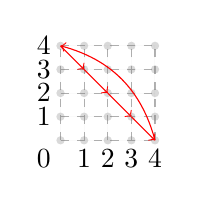
\begin{tikzpicture}[scale=0.3]
    % grid
    \draw[dashed,fill=gray,opacity=.3]  (0,0) grid (4,4);
    % labels
    \foreach \x in {1,...,4} { \node [anchor=north] at (\x,0) {\x}; }
    \foreach \y in {1,...,4} { \node [anchor=east] at (0,\y) {\y}; }
    \node [anchor=north east] at (0,0) {0};
    % vertices
    \foreach \x in {0,...,4} {
        \foreach \y in {0,...,4} {
            \node at (\x,\y) [circle,inner sep=0pt,minimum size=3pt,fill=gray,opacity=.3] {};
        }
    }
    % path
\draw [->,red] (4,0) to [bend right=30] (0,4);
\draw [->,red] (0,4) -- (1,3);
\draw [->,red] (1,3) -- (2,2);
\draw [->,red] (2,2) -- (3,1);
\draw [->,red] (3,1) -- (4,0);
\end{tikzpicture}
\caption{Quot./Rem.}
\label{sfig:Quot./Rem.}
\end{subfigure}
\hfill
\begin{subfigure}{.225\textwidth}
\centering
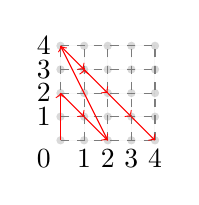
\begin{tikzpicture}[scale=0.3]
    % grid
    \draw[dashed,fill=gray,opacity=.5]  (0,0) grid (4,4);
    % labels
    \foreach \x in {1,...,4} { \node [anchor=north] at (\x,0) {\x}; }
    \foreach \y in {1,...,4} { \node [anchor=east] at (0,\y) {\y}; }
    \node [anchor=north east] at (0,0) {0};
    % vertices
    \foreach \x in {0,...,4} {
        \foreach \y in {0,...,4} {
            \node at (\x,\y) [circle,inner sep=0pt,minimum size=3pt,fill=gray,opacity=.3] {};
        }
    }
    % path
\draw [->,red] (0,0) -- (0,2);
\draw [->,red] (0,2) -- (1,1);
\draw [->,red] (1,1) -- (2,0);
\draw [->,red] (2,0) -- (0,4);
\draw [->,red] (0,4) -- (1,3);
\draw [->,red] (1,3) -- (1,3);
\draw [->,red] (1,3) -- (2,2);
\draw [->,red] (2,2) -- (3,1);
\draw [->,red] (3,1) -- (4,0);
\end{tikzpicture}
\caption{Square root}
\label{sfig:Square root}
\end{subfigure}
\hfill
    \begin{subfigure}{.225\textwidth}
    \centering
    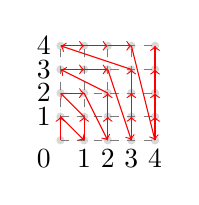
\begin{tikzpicture}[scale=0.3]
        % grid
        \draw[dashed,fill=gray,opacity=.5]  (0,0) grid (4,4);
        % labels
        \foreach \x in {1,...,4} { \node [anchor=north] at (\x,0) {\x}; }
        \foreach \y in {1,...,4} { \node [anchor=east] at (0,\y) {\y}; }
        \node [anchor=north east] at (0,0) {0};
        % vertices
        \foreach \x in {0,...,4} {
            \foreach \y in {0,...,4} {
                \node at (\x,\y) [circle,inner sep=0pt,minimum size=3pt,fill=gray,opacity=.3] {};
            }
        }
        % path
        \draw [->,red] (0,0) -- (0,1);
        \draw [->,red] (0,1) -- (1,0);
        \draw [->,red] (1,0) -- (1,1);
        \draw [->,red] (1,1) -- (0,2);
        \draw [->,red] (0,2) -- (1,2);
        \draw [->,red] (1,2) -- (2,0);
        \draw [->,red] (2,0) -- (2,1);
        \draw [->,red] (2,1) -- (2,2);
        \draw [->,red] (2,2) -- (0,3);
        \draw [->,red] (0,3) -- (1,3);
        \draw [->,red] (1,3) -- (2,3);
        \draw [->,red] (2,3) -- (3,0);
        \draw [->,red] (3,0) -- (3,1);
        \draw [->,red] (3,1) -- (3,2);
        \draw [->,red] (3,2) -- (3,3);
        \draw [->,red] (3,3) -- (0,4);
        \draw [->,red] (0,4) -- (1,4);
        \draw [->,red] (1,4) -- (2,4);
        \draw [->,red] (2,4) -- (3,4);
        \draw [->,red] (3,4) -- (4,0);
        \draw [->,red] (4,0) -- (4,1);
        \draw [->,red] (4,1) -- (4,2);
        \draw [->,red] (4,2) -- (4,3);
        \draw [->,red] (4,3) -- (4,4);
    \end{tikzpicture}
    \caption{\lstinline|mkpair|}
    \label{sfig:mkpair}
\end{subfigure}
\caption{Paths in $ \NN^2 $ that generate algorithms in \lstinline|rpp|.}
\label{fig:functions as paths}
\end{figure}

\paragraph{Cantor (Un-)Pairing}
The standard definition of Cantor Pairing $\rppcp : \NN^2 \to \NN$ and Un-pairing $\rppcu : \NN \to \NN^2$, two bijections one inverse of the other, is:
\begin{align}
\label{align: cp analitically}
\rppcp(x,y) & = \sum_{i=1}^{x+y}i + x = \frac{(x + y)(x + y + 1)}{2} + x
\\
\label{align: cu analitically}
\rppcu(n)  & = \left( n - \frac{i(1+i)}{2}, \frac{i(3+i)}{2} - n \right)
\enspace ,
\end{align}
where $i = \left\lfloor \frac{\sqrt{8n + 1} - 1}{2} \right\rfloor $.

\begin{figure}
\begin{subfigure}{.975\textwidth}
    \centering
\scalebox{.75}{
    $\begin{NiceMatrix}
        x &\bloch{2-1}{\mbox{\lstinline|inc|}}&x&\bloch{1-1}{\mbox{\lstinline|Id 1|}}&x&\bloch{1-1}{\mbox{\lstinline|Id 1|}}&\bloch{2-1}{\mbox{\lstinline|dec|}}&x& \bloch{4-1}{\rpprewire{0,3,1}} &\bloch{2-1}{\mbox{\lstinline|inc|}} &\bloch{1-1}{\mbox{\lstinline|Id 1|}} & x
        \\
        y && x + y & \bloch{3-1}{
            \mbox{\lstinline|It(Su;;inc)|}
            %            \rppIt[\rppSu \rppCo \rppinc]
        } & x + y& \bloch{2-1}{\mbox{\lstinline|dec|}} && y&&& \bloch{2-1}{\mbox{\lstinline|Sw|}} & y
        \\
        0 &                      & 0     &                     & x + y                &                      &                      & 0                    &                      &                      &                     & \sum_{i=1}^{x + y} i + x
        \\
        0 &                      & 0     &                     & \sum_{i=1}^{x + y} i &                      &                      & \sum_{i=1}^{x + y} i &                      &                      &                     & 0
    \end{NiceMatrix}$
}
    \caption{Function \lstinline|cp_in|}
    \label{sfig:cp input}
\end{subfigure}
\\ \\ \\
\begin{subfigure}{.975\textwidth}
\centering
\scalebox{.55}{
    $\begin{NiceMatrix}
        & x &\bloch{1-1}{\mbox{\lstinline|Id 1|}}& x & \bloch{3-1}{\rpprewire{2,0,1}} & 1 & \bloch{3-1}{
            \mbox{\lstinline|If(Su‖Pr)(Su;;Sw)(Id 1)|}
%            \rppIf[\boldsymbol{\rppSu \rppPa \rppPr}, \mbox{\lstinline|Su;;Sw|}, \ \rppId_1]
        } & 1     & \bloch{2-1}{
        \mbox{\lstinline|Sw|}
%        \rppSw
        } & x + 1 & \bloch{2-1}{
        \mbox{\lstinline|If(Pr)(Id 1)(Id 1)|}
%        \rppIf[\boldsymbol{\rppPr}, \rppId_1, \rppId_1]
        } & x + 1 &\bloch{1-1}{\mbox{\lstinline|Id 1|}} & x + 1 \\
        & \yb & \bloch{2-1}{
        \mbox{\lstinline|If(Su)(Id 1)(Id 1)|}
        %            \rppIf[\boldsymbol{\rppSu}, \rppId_1, \rppId_1]
        } & \yb &&x&& x + 1 &                     & 1     &                                                              & 0     & \bloch{2-1}{
        \mbox{\lstinline|Sw|}
%        \rppSw
        } & \yb - 1 \\
        & 0&&1&&\yb&& \yb - 1 && \yb - 1 && \yb - 1 && 0
    \end{NiceMatrix}$
}
\caption{Function \lstinline|step[Su;;Sw]|: detailed behavior with $ \yb > 0 $. }
\label{sfig:cu step y > 0}
\end{subfigure}
\\ \\ \\
\begin{subfigure}{.975\textwidth}
\centering
\scalebox{.55}{
$\begin{NiceMatrix}
    & x &\bloch{1-1}{\mbox{\lstinline|Id 1|}}& x & \bloch{3-1}{\rpprewire{2,0,1}} & 0 & \bloch{3-1}{
    \mbox{\lstinline|If(Su‖Pr)(Su;;Sw)(Id 1)|}
    %    \rppIf[\rppSu \rppPa \rppPr, \mbox{\lstinline|Su;;Sw|} , \ \rppId_1]
    } & 0     & \bloch{2-1}{
    \mbox{\lstinline|Sw|}
    %    \rppSw
    } & \yr & \bloch{2-1}{
        \mbox{\lstinline|If(Pr)(Id 1)(Id 1)|}
%        \rppIf[\rppPr, \boldsymbol{\rppId_1}, \rppId_1]
    } & \yr & \bloch{1-1}{\mbox{\lstinline|Id 1|}} & \yr
    \\
    & \yr & \bloch{2-1}{
        \mbox{\lstinline|If(Su)(Id 1)(Id 1)|}
%        \rppIf[\rppSu, \boldsymbol{\rppId_1}, \rppId_1]
    } & \yr && x &&\yr&&0&&0&\bloch{2-1}{
        \mbox{\lstinline|Sw|}
%        \rppSw
   } & x + 1
    \\
    & 0 && 0 && \yr && x + 1 && x + 1 && x + 1 && 0
\end{NiceMatrix}$
}
\caption{Function \lstinline|step[Su;;Sw]|: detailed  behavior with $ \yr = 0 $. }
\label{sfig:cu step y = 0}
\end{subfigure}
\\ \\ \\
\begin{subfigure}{.975\textwidth}
\centering
\scalebox{.82}{
$\begin{NiceMatrix}
     \rppcp(x,y)
      & \bloch{4-1}{\mbox{\lstinline|It step[Su;;Sw]| }} &
      \rppcp(x,y)\\
    0 &                      & x \\
    0 &                      & y \\
    0 &                      & 0
\end{NiceMatrix}$
}
\caption{Function \lstinline|cu_in|}
\label{sfig:cu input}
\end{subfigure}
\\ \\ \\
\begin{subfigure}{.665\textwidth}
    \centering
\scalebox{.82}{
    $ \begin{NiceMatrix}
        x & \bloch{4-1}{\mbox{\lstinline|cp_in|}} & x           & \bloch{3-1}{\rpprewire{2,0,1}} & \rppcp(x,y) & \bloch{4-1}{\mbox{\lstinline|cu_in⁻¹|}} & \rppcp(x,y) \\
        y &                       & y           &                      & x           &                            & 0           \\
        0 &                       & \rppcp(x,y) &                      & y           &                            & 0           \\
        0 &                       & 0           &                      & 0           &                            & 0           \\
    \end{NiceMatrix}
    $
}
\caption{The function \lstinline|cp|}
\label{sfig:cp}
\end{subfigure}
\hfill
\begin{subfigure}{.325\textwidth}
\centering
\scalebox{.82}{
    $ \begin{NiceMatrix}
        n & \bloch{4-1}{\mbox{\lstinline|cp⁻¹|}} & \rppcu_1(n)    \\
        0 &                      & \rppcu_2(n)         \\
        0 &                      & 0 \\
        0 &                      & 0
    \end{NiceMatrix} $
}
\caption{The function \lstinline|cu|}
\label{sfig:cu}
\end{subfigure}
\caption{Cantor Pairing and Un-pairing.}
\label{fig:Cantor}
\end{figure}

Figure~\ref{fig:Cantor} has all we need to define Cantor Pairing \lstinline|cp:rpp|, and Un-pairing \lstinline|cu:rpp|.
In Figure~\ref{sfig:cp input}, \lstinline|cp_in| is the natural algorithm in \lstinline|rpp| to implement~\eqref{align: cp analitically}. As expected, the input pair $(x,y)$ is part of \lstinline|cp_in| output, a fact that the suffix ``\lstinline|_in|'' recalls in the name of the function. In order to drop $(x,y)$ from the output of \lstinline|cp_in|, and to obtain \lstinline|cp| as in Figure~\ref{sfig:cp}, we apply {\it Bennett's trick} using \lstinline|cu_in⁻¹|, i.e.\@ the inverse of \lstinline|cu_in|, whose definition is completely new, as compared to the corresponding one defined previously in \cite{DBLP:journals/tcs/PaoliniPR20}. The intuition behind \lstinline|cu_in| is as follows. Let us fix any point $ (x, y) \in \NN^2 $. We can realize that, starting from the origin, if we follow as many steps as the value $ \rppcp(x, y) $ in Figure~\ref{sfig:cantor as a path}, we stop exactly at $ (x,y) $. A standard functional notation for the function that, given the current point $ (x,y) $, identifies the next one to move to in the path of Figure~\ref{sfig:cantor as a path} is:
\begin{align*}
%    \label{align:next function}
    \operatorname{step}(x,y) & =
    \begin{cases} (x+1,y-1) &  y > 0 \\ (0, x+1) &   y = 0 \end{cases}
    \enspace .
\end{align*}
We implement $ \operatorname{step}(x,y) $ in \lstinline|rpp| as \lstinline|step[Su;;Sw]|. Figures~\ref{sfig:cu step y > 0}, and~\ref{sfig:cu step y = 0} represent two runs of \lstinline|step[Su;;Sw]| to give visual evidence that \lstinline|step[Su;;Sw]| implements $\operatorname{step}(x,y)$. Colored occurrences of $ y $ show the relevant part of the computational flow. Note that we cannot implement $ \operatorname{step}(x,y) $ by using the conditional directly on $y$, because in the computation we also want to modify the value of $y$. Finally, as soon as we get \lstinline|cu_in| by iterating \lstinline|step[Su;;Sw]| as in Figure~\ref{sfig:cu input}, we can define \lstinline|cp| (Figure~\ref{sfig:cp}), and \lstinline|cu| (Figure~\ref{sfig:cu}).

\begin{figure}
    \begin{subfigure}{.475\linewidth}
        \centering
\scalebox{.85}
{        $ \begin{NiceMatrix}
            m & \bloch{5-1}{\mbox{\lstinline|It step[Sw‖Su]|}} & m         \\
            0 &                      & r         \\
            n &                      & n + 1 - r \\
            0 &                      & 0         \\
            0 &                      & q         \\
        \end{NiceMatrix} $
}        \caption{Function that computes $ q $ and $ r $ such that $m = q(n + 1) + r$. We obtain it by iterating \lstinline|step[Sw‖Su]|.}
        \label{sfig:div}
    \end{subfigure}
    \hfill
    \begin{subfigure}{.475\linewidth}
        \centering
 \scalebox{.85}
 {       $\begin{NiceMatrix}
            n & \bloch{5-1}{\mbox{\lstinline|It step[Su;;Su;;Sw‖Su]|}} & n      \\
            0 &                       & r                      \\
            0 &                       & 2 \floor{\sqrt{n}} - r \\
            0 &                       & 0                      \\
            0 &                       & \floor{\sqrt{n}}       \\
        \end{NiceMatrix}
        $
}
        \caption{Function that computes $ \floor{\sqrt{n}}$ and $ r = n - \floor{\sqrt{n}}^2 $. We obtain it by iterating \lstinline|step[Su;;Su;;Sw‖Su]|.}
        \label{sfig:sqrt}
    \end{subfigure}%
\caption{Quotient/Reminder and Square root.}
\end{figure}

%=============================
\paragraph{Quotient and reminder}
%In defining the function $\rppcui$ we framed it as a "path" in a two-dimensional grid.
Let us focus on the path in Figure~\ref{sfig:Quot./Rem.}.
It starts at $(0,n)$ (with $ n = 4 $), and, at every step, the next point is in \emph{direction} $(+1,-1)$. When it reaches $(n,0)$ (with $ n = 4 $), instead of jumping to $(0,n+1)$, as in Figure~\ref{sfig:cantor as a path}, it lands again on $(0,n)$. The idea is to keep looping on the same diagonal. This behavior can be achieved by iterating \lstinline|step[Sw‖Su]|. Figure~\ref{sfig:div} shows that we are doing modular arithmetic.
Globally, it takes $n+1$ steps from $ (0,n) $ to itself by means of \lstinline|step[Sw‖Su]|.
Specifically, if we assume we have performed $m$ steps along the diagonal, and we are at point $ (x,y) $, we have that $x \equiv m \pmod{n+1}$ and $0 \le x \le n$.
So, if we increase a counter by one each time we reset our position to $(0,n)$ we can calculate quotient and reminder.

%====================
\paragraph{Truncated Square root}
Let us focus on the path in Figure~\ref{sfig:Square root}.
It starts at $(0,0)$. Whenever it reaches $(x,0)$ it jumps to $(0,x+2)$, otherwise the next point is in \emph{direction} $(+1,-1)$.
The behavior can be achieved by iterating \lstinline|step[Su;;Su;;Sw‖Su]| as in Figure~\ref{sfig:sqrt}.
In order to compute $ \floor{\sqrt{n}} $, besides implementing the above path, the function \lstinline|step[Su;;Su;;Sw‖Su]| counts in $ k $ the number of jumps occurred so far along the path. In particular, starting from $ (0,0) $, the first jump occurs in the first step; the next one in the $(1+3)$th, then the $(1+3+5)$th, then the $(1+3+5+7)$th etc. Since we know that $1 + 3 + \dots + (2k - 1) = k^2$ for any $k$, letting $n$ be the number of iterations (and hence the numbers of steps) we have that $k$ is such that $k^2 \le n < (k+1)^2$; i.e. $k = \floor{\sqrt{n}}$.

\begin{remark}
The value $2 \floor{\sqrt{n}} - r$ can be canceled out by adding $r$, and subtracting $\floor{\sqrt{n}}$ twice.
What we \emph{cannot} eliminate is the ``remainder'' $r = n - \left\lfloor \sqrt{n} \right\rfloor^2$ because the \emph{function} Square root
cannot be inverted in $ \ZZ $, and the algorithm cannot forget it.
\end{remark}

\paragraph{The $\rppmkpair$ function}
Figure~\ref{sfig:mkpair} shows the behavior of the function $\rppmkpair$.
It is very similar to the one of $\rppcp$, but it uses an alternative algorithm described in \cite{Carneiro19}.
Here we do not describe it in detail because it's just a composition of sums, products and square roots,
just discussed here above.

\subsection{A note on the mechanization of proofs}
We recall once more that everything defined above has been proved correct in \LEAN (see \cite{MalettoRPPLEAN2021} for the details).
For example, once defined \lstinline|sqrt| in \LEAN, the following lemma:
\begin{lstlisting}
   lemma sqrt_def (n : ℕ) (X : list ℤ) :
     ‹sqrt›(n::0::0::0::0::X) =
              n::(n-√n*√n)::(√n+√n-(n-√n*√n))::0::√n::X
\end{lstlisting}
shows that \lstinline|sqrt| behaves as expected, for any \lstinline|n|.

In order to prove the here above lemma, or similar ones, we make use of the {\it tactic} \lstinline|simp|, i.e.\@ a \LEAN command that builds proofs. The tactic \lstinline|simp| can automatically simplify expressions until trivial identities show up. What is meant by ``simplify'' is that theorems which state an equality with form \texttt{Left\_hand\_side = Right\_hand\_side}, like in \lstinline|sqrt_def|,  can be marked with the attribute \lstinline|@[simp]|; the very useful consequence is that every time \lstinline|simp| is invoked in a subsequent proof, if the equality to be proved contains an instance of \texttt{Left\_hand\_side}, then it will be substituted with \texttt{Right\_hand\_side}, often making it simpler to conclude a proof.

So, \lstinline|@[simp]| introduces an incremental and quite handy mechanism to automate proofs: the more available proofs exist, the more we can, in principle, label as \lstinline|@[simp]|, widening the possibility to automatically prove further properties.



%=====================
\section{Proving in \LEAN that \RPP is \PRF-complete}
\label{section:The UPRF-completeness of RPP}
We formally show in \LEAN that the class of functions we can express as (algorithms) in \lstinline|rpp| contains at least the class \PRF of Primitive Recursive Functions; we say that ``\lstinline|rpp| is \PRF-complete''. The definition of \PRF that we take as reference is one of the two available in \LEAN \MATHLIB library. Once recalled and commented it briefly, we shall proceed with the main aspects of the \PRF-completeness of \lstinline|rpp|.


\begin{figure}
\begin{lstlisting}[basicstyle=\small]
inductive primrec:(ℕ → ℕ) → Prop
| zero: primrec (λ (n:ℕ), 0)
| succ: primrec succ
| left: primrec (λ (n:ℕ), (unpair n).fst)
| right: primrec (λ (n:ℕ), (unpair n).snd)
| pair {F G}: primrec F → primrec G → primrec (λ (n:ℕ), mkpair (F n) (G n))
| comp {F G}: primrec F → primrec G → primrec (λ (n:ℕ), F (G n))
| prec {F G}: primrec F → primrec G → primrec
(unpaired (λ (z n:ℕ), nat.rec (F z) (λ (y IH:ℕ), G (mkpair z (mkpair y IH))) n))
\end{lstlisting}
\caption{\lstinline|primrec| defines \PRF in \MATHLIB of \LEAN.}
\label{fig: primrec}
\end{figure}


%=====================
\subsection{Primitive Recursive Functions \texttt{primrec} in \MATHLIB }
\label{section:Unary Primitive Recursive Functions}

Figure~\ref{fig: primrec} recalls the definition of \PRF from \cite{Carneiro-primrecMathlib} available in \MATHLIB that we take as reference. It is an inductively defined \lstinline|Prop|osition \lstinline|primrec| that requires a \emph{unary} function with type \lstinline|ℕ → ℕ| as argument. Specifically, \lstinline|primrec| is the least collection of functions \lstinline|ℕ → ℕ| with a given set of base elements, closed under some composition schemes.

\paragraph{Base functions of {\normalfont \texttt{primrec}}}
The \emph{constant} function \lstinline|zero| yields \lstinline|0| on every of its inputs.
The \lstinline|succ|\emph{essor} gives the natural number next to the one taken as input.
The two \emph{projections} \lstinline|left|, and \lstinline|right| take an argument \lstinline|n|, and extract a left, or a right, component from it as \lstinline|n| was the result of pairing two values \lstinline|x,y:ℕ|. The functions that \lstinline|primrec| relies on to encode/decode pairs on natural numbers as a single natural one are \lstinline|mkpair:ℕ → ℕ → ℕ|, and \lstinline|unpair:ℕ → ℕ × ℕ|. The first one builds the value \lstinline|mkpair x y|, i.e. the number of steps from the origin to reach the point with coordinates \lstinline|(x,y)| in the path of Figure~\ref{sfig:mkpair}. The function \lstinline|unpair:ℕ → ℕ × ℕ| takes the number of steps to perform on the same path. Once it stops, the coordinates of that point are the two natural numbers we are looking for. So, \lstinline|mkpair|/\lstinline|unpair| are an alternative to Cantor Pairing/Un-pairing.

\paragraph{Composition schemes}
Three schemes exist in \lstinline|primrec|, each depending on parameters \lstinline|f,g:primrec|.
The scheme \lstinline|pair| builds the function that, taken a value \lstinline|n:ℕ|, gives the unique value in \lstinline|ℕ| that encodes the pair of values \lstinline|F n|, and \lstinline|G n|; everything we might pack up by means of \lstinline|pair|, we can unpack with \lstinline|left|, and \lstinline|right|.

The scheme \lstinline|comp| composes \lstinline|F,G:primrec|.

The \emph{primitive recursion} scheme \lstinline|prec| can be ``unfolded'' to understand how it works. This reading will ease the description of how to encode it in \lstinline|rpp|.
Let \lstinline|F|, \lstinline|G| be two elements of \lstinline|primrec|. We see \lstinline|prec| as encoding the function:
\begin{align}
\label{align:function H}
H[\mbox{\lstinline|F|},\mbox{\lstinline|G|}](x) & =
R[\mbox{\lstinline|G|}]\big( \mbox{\lstinline|F|} \big((x)_1 \big) , (x)_2 \big)
\end{align}
where:
(i) $(x)_1$ denotes \lstinline|(unpair| x\lstinline|).fst|,
(ii) $(x)_2$ denotes \lstinline|(unpair| x\lstinline|).snd|,
and
(iii) $R [\mbox{\lstinline|G|}] $ behaves as follows:
\begin{equation}
\label{equation:function R}
\begin{aligned}
    R[\mbox{\lstinline|G|}](z,0) & = z \\
    R[\mbox{\lstinline|G|}](z,n+1) &
    = \mbox{\lstinline|G|} \big(
      \gl z, \gl n, R[\mbox{\lstinline|G|}](z,n) \gr \gr
      \big)
   \enspace ,
\end{aligned}
\end{equation}
defined using the built-in recursive scheme \lstinline|nat.rec| on \lstinline|ℕ|, and $ \gl a, b \gr $ denotes $ (\mbox{\lstinline|mkpair|}\ a\ b) $.

%=================
\subsection{The main point of the proof}
In order to formally state what we mean for \lstinline|rpp| to be \PRF-complete, in \LEAN we need to say when, given \lstinline|F:ℕ → ℕ|, we can \emph{encode} it by means of some \lstinline|f:rpp|. This is done by means of the following definition:
\begin{lstlisting}
 def encode (F:ℕ → ℕ) (f:rpp) :=
     ∀ (z:ℤ) (n:ℕ), ‹f› (z::n::repeat 0 (f.arity-2))
                            = (z+(F n))::n::repeat 0 (f.arity-2)
\end{lstlisting}
which says that, fixed \lstinline|F:ℕ → ℕ|, and \lstinline|f:rpp|, the statement \lstinline|(encode F f)| holds if the evaluation of \lstinline|‹f›|, applied to any argument \lstinline|(z::n::0::...::0)| with as many occurrences of trailing \lstinline|0|s as \lstinline|f.arity-2|, gives a list with form \lstinline|((z+(F n))::n::0::...::0)| such that:
\begin{enumerate}
    \item[(i)]
    the first element is the original value \lstinline|z| increased with the result \lstinline|(F n)| of the function we want to encode;
    \item[(ii)]
    the second element is the initial \lstinline|n|;
    \item[(iii)]
    trailing \lstinline|0|s are again as many as \lstinline|f.arity-2|.
\end{enumerate}
In \LEAN we can prove:
\begin{lstlisting}
    theorem completeness (F:ℕ → ℕ):
                primrec F → ∃ f:rpp, encode F f
\end{lstlisting}
which says that we know how to build \lstinline|f:rpp| which \lstinline|encode|s \lstinline|F|, for every well formed \lstinline|F:ℕ → ℕ|, i.e.\@ such that \lstinline|primrec F| holds.

The proof proceeds by induction on the proposition \lstinline|primrec|, which generates 7 sub-goals. We illustrate the main arguments to conclude the most interesting case which requires to encode the composition scheme \lstinline|prec|.

\begin{remark}
Many aspects of the proof that we here detail out, ``forced'' by \LEAN, so to say, were simply missing in the original \PRF-completeness proof for \RPP in \cite{DBLP:journals/tcs/PaoliniPR20}.
\qed
\end{remark}

The inductive hypothesis to show that we can encode \lstinline|prec| is that, for any given \lstinline|F,G:ℕ → ℕ| such that \lstinline|(primrec F):Prop|, and \lstinline|(primrec G):Prop|, both \lstinline|f,g:rpp| exist such that \lstinline|(encode F f)|, and \lstinline|(encode G g)| hold. This means that both:
\begin{align*}
\mbox{\lstinline|f|}\ (z\mbox{\lstinline|::|}n\mbox{\lstinline|::|}\boldsymbol{0})
& = (z+\mbox{\lstinline|F|}\ n)\mbox{\lstinline|::|}n\mbox{\lstinline|::|}\boldsymbol{0}
\\
\mbox{\lstinline|g|}\ z\mbox{\lstinline|::|}n\mbox{\lstinline|::|}\boldsymbol{0}
& = (z+\mbox{\lstinline|G|}\ n)\mbox{\lstinline|::|}n\mbox{\lstinline|::|}\boldsymbol{0}
\end{align*}
hold, where $ \boldsymbol{0} $ stands for a sufficiently long list of $ 0 $s.
%%%% ---- do not remove this line
\begin{figure}
\newcommand{\bz}{\boldsymbol{0}}
\newcommand{\by}{\boldsymbol{y}}
\newcommand{\bid}{\bloch{1-1}{\mbox{\lstinline|Id 1|}}}
\newcommand{\bidt}{\bloch{2-1}{\mbox{\lstinline|Id 2|}}}
\newcommand{\bsw}{\bloch{2-1}{\mbox{\lstinline|Sw|}}}
\newcommand{\bpi}{\bloch{3-1}{\mbox{\lstinline|H[f,g]|}}}
\newcommand{\binc}{\bloch{2-1}{\mbox{\lstinline|inc|}}}
\newcommand{\bup}{\bloch{5-1}{\mbox{\lstinline|unpair|}}}
\newcommand{\bpiinv}{\bloch{3-1}{\mbox{\lstinline|H[f,g]⁻¹|}}}
\newcommand{\bff}{\bloch{5-1}{\mbox{\lstinline|f|}}}
\newcommand{\bfg}{\bloch{3-1}{\mbox{\lstinline|g|}}}
\newcommand{\bre}{\bloch{4-1}{\rpprewire{0,2,3,1}}}
\newcommand{\brs}{\bloch{6-1}{\rpprewire{0,1,4,3,5,2}}}
\newcommand{\brc}{\bloch{6-1}{\rpprewire{5,0}}}
\newcommand{\bipsg}{\bloch{5-1}{\mbox{\lstinline|It R[g]|}}}
\begin{subfigure}{.95\textwidth}
\centering
\scalebox{.9}
{$\begin{NiceMatrix}
 z  &\bpi&\binc&\bpiinv&z + H[\mbox{\lstinline|F|},\mbox{\lstinline|G|}] (n)\\
 n  &    &    &       &n\\
 \bz&    &    &       &\bz
 \end{NiceMatrix}$}
\caption{The function \lstinline|prec[f,g]:rpp|.}
\label{sfig:prec[f,g]}
\end{subfigure}
\\ \\ \\
\begin{subfigure}{.95\textwidth}
\centering
\scalebox{.9}{
$\begin{NiceMatrix}
 z  &\bid&\bre&\bidt&\brs&\bid  &\brc& H[\mbox{\lstinline|F|},\mbox{\lstinline|G|}] (n)  \\
 n  &\bup&    &     &    &\bipsg&    & z      \\
 0  &    &    &\bff &    &      &    & (n)_2  \\
 0  &    &    &     &    &      &    & s      \\
 0  &    &    &     &    &      &    & (n)_1  \\
 0  &    &    &     &    &      &    & (n)_2  \\
 \bz&    &    &     &    &      &    & \bz
\end{NiceMatrix}$
 }
\caption{The function \lstinline|H[f,g]| with parameters \lstinline|f, g|.}
\label{sfig:precfwd[f,g]}
\end{subfigure}
\caption{Encoding \lstinline|prec| of Figure~\ref{fig: primrec} in \lstinline|rpp|.}
\label{fig:composing encode prec}
\end{figure}
%%%% ---- do not remove this line
Moreover, Figure~\ref{sfig:prec[f,g]}, in which the assumption is that $ z = 0 $, defines \lstinline|prec[f,g]:rpp| such that:
\begin{enumerate}
    \item[(i)]
    \lstinline|(encode (prec F G) prec[f,g]):Prop| holds, and
    \item [(ii)]
    \lstinline|H[f,g]| encodes $ H[\mbox{\lstinline|F|},\mbox{\lstinline|G|}]$
\end{enumerate}
as in~\eqref{align:function H}.
Finally, the term \lstinline|It R[g]| in \lstinline|H[f,g]| encodes~\eqref{equation:function R} by iterating \lstinline|R[g]| from the initial value given by \lstinline|f|.

Figure~\ref{fig:main step RPF-completeness} splits the definition of \lstinline|R[g]| into three logical parts.
Figure~\ref{sfig:encode prec 1st step} packs everything up by means of \lstinline|mkpair| to build the argument $ R[\mbox{\lstinline|G|}](z,n) $ of \lstinline|g|; by induction we get
$ R[\mbox{\lstinline|G|}](z,n+1) $.
In Figure~\ref{sfig:encode prec 2nd step}, \lstinline|unpair| unpacks $ \gl z, \gl n, R[\mbox{\lstinline|G|}](z,n) \gr \gr $ to expose its components to the last part.
Figure~\ref{sfig:encode prec 3rd step} both increments $ n $, and packs $ R[\mbox{\lstinline|G|}](z,n) $ into $ s $, by means of \lstinline|mkpair|, because $ R[\mbox{\lstinline|G|}](z,n) $ has become useless once obtained $ R[\mbox{\lstinline|G|}](z,n+1) $ from it. Packing $ R[\mbox{\lstinline|G|}](z,n) $ into $ s $, so that we can eventually recover it, \emph{is mandatory}. We cannot ``replace'' $ R[\mbox{\lstinline|G|}](z,n) $ with $ 0 $ because that would not be a reversible action.

\begin{remark}
The function \lstinline|cp| in Figure~\ref{sfig:cp} can replace \lstinline|mkpair| in Figure~\ref{sfig:encode prec 3rd step} as a bijective map $ \NN^2$ into $\NN$. Indeed, the original \PRF-completeness of \RPP relies on \lstinline|cp|. We favor \lstinline|mkpair| to take the most out of \MATHLIB.
\qed
\end{remark}



\begin{figure}
    \begin{subfigure}{.975\textwidth}
        \centering
        \scalebox{.9}{
            $\begin{NiceMatrix}
                s&\bloch{2-1}{\mbox{\lstinline|Id 2|}}&\bloch{1-1}{\mbox{\lstinline|Id 1|}}& s &\bloch{1-1}{\mbox{\lstinline|Id 1|}}&\bloch{1-1}{\mbox{\lstinline|Id 1|}}& s
                \\
                z&& \bloch{5-1}{\mbox{\lstinline|mkpair|}} & \gl z, \gl n, R[\mbox{\lstinline|G|}](z,n) \gr \gr & \bloch{2-1}{\mbox{\lstinline|Sw|}} & \bloch{5-1}{\mbox{\lstinline|g|}}&R[\mbox{\lstinline|G|}](z,n+1)
                \\
                n& \bloch{4-1}{\mbox{\lstinline|mkpair|}} &&0&&& \gl z, \gl n, R[\mbox{\lstinline|G|}](z,n) \gr \gr
                \\
                R[\mbox{\lstinline|G|}](z,n) &                         &                         & 0                                       &                     &                & 0                                       \\
                0                 &                         &                         & 0                                       &                     &                & 0                                       \\
                \boldsymbol{0}    &                         &                         & \boldsymbol{0}                          &                     &                & \boldsymbol{0}                          \\
            \end{NiceMatrix}$
        }
        \caption{Build the argument $ \gl z, \gl n, R[\mbox{\lstinline|G|}](z,n) \gr \gr $ of \lstinline|g|.}
        \label{sfig:encode prec 1st step}
    \end{subfigure}
    \\ \\ \\
    \begin{subfigure}{.975\textwidth}
        \centering
        \scalebox{.9}{
            $   \begin{NiceMatrix}
                s &\bloch{2-1}{\mbox{\lstinline|Id 2|}}&\bloch{3-1}{\mbox{\lstinline|Id 3|}}&s& \bloch{5-1}{\rpprewire{2,3,1,0,4}} & z                   \\
                R[\mbox{\lstinline|G|}](z,n+1)                     &                         &                         & R[\mbox{\lstinline|G|}](z,n+1) &                            & n                   \\
                \gl z, \gl n, R[\mbox{\lstinline|G|}](z,n) \gr \gr & \bloch{4-1}{\mbox{\lstinline|unpair|}} &                         & z                   &                            & R[\mbox{\lstinline|G|}](z,n+1) \\
                0                                       &                         & \bloch{3-1}{\mbox{\lstinline|unpair|}} & n                   &                            & s                   \\
                0                                       &                         &                         & R[\mbox{\lstinline|G|}](z,n)   &                            & R[\mbox{\lstinline|G|}](z,n)   \\
                \boldsymbol{0}                          &                         &                         & \boldsymbol{0}      &                            & \boldsymbol{0}      \\
            \end{NiceMatrix}$
        }
        \caption{Unpack $ \gl z, \gl n, R[\mbox{\lstinline|G|}](z,n) \gr \gr $ to let its elements available.}
        \label{sfig:encode prec 2nd step}
    \end{subfigure}
    \\ \\ \\
    \begin{subfigure}{.975\textwidth}
        \centering
        \scalebox{.9}{
            $    \begin{NiceMatrix}
                z&\bloch{1-1}{\mbox{\lstinline|Id 1|}}& z& \bloch{4-1}{\rpprewire{3,0,1,2}} & s'                  \\
                n                   & \bloch{1-1}{\mbox{\lstinline|Su|}}     & n + 1               &                         & z                   \\
                R[\mbox{\lstinline|G|}](z,n+1) &\bloch{1-1}{\mbox{\lstinline|Id 1|}} & R[\mbox{\lstinline|G|}](z,n+1) &                         & n + 1               \\
                s                   & \bloch{3-1}{\mbox{\lstinline|mkpair|}} & s'                  &                         & R[\mbox{\lstinline|G|}](z,n+1) \\
                R[\mbox{\lstinline|G|}](z,n)   &                         & 0                   &                         & 0                   \\
                \boldsymbol{0}      &                         & \boldsymbol{0}      &                         & \boldsymbol{0}      \\
            \end{NiceMatrix}$
        }
        \caption{Increment $ n $, and store $ R[\mbox{\lstinline|G|}](z,n) $ to keep the whole process reversible.}
        \label{sfig:encode prec 3rd step}
    \end{subfigure}
    \caption{Encoding $ R[\mbox{\lstinline|G|}] $ in~\eqref{equation:function R} as \lstinline|R[g]:rpp|.}
    \label{fig:main step RPF-completeness}
\end{figure}

%=====================
\section{Proving in \LEAN that \RPP is \PRF-sound}
\label{section:Each RPP is PRF}

We formally show in \LEAN that every function we can express as (algorithm) in \lstinline|rpp| can be expressed as an element of \PRF, the class of Primitive Recursive Functions; we say that ``\lstinline|rpp| is \PRF-sound''.
This means that, through a suitable embedding of \lstinline|list ℤ| in \lstinline|ℕ| and thus seeing each \lstinline|‹f›:list ℤ → list ℤ| as a function of type \lstinline|ℕ → ℕ|, this is always primitive recursive. In \LEAN terms, we can prove:
\begin{lstlisting}
        theorem rpp_primrec (f:rpp) : primrec ‹f›
\end{lstlisting}
As far as we know, no full proof of this fact was present before, \cite{Paolini2018NGC} included. In order to show it, we make heavy use of previously established theorems present in \LEAN \MATHLIB library.

%%%%
\subsection{The extended definition of {\normalfont \texttt{primrec}} in {\normalfont \MATHLIB}}
Section~\ref{section:The UPRF-completeness of RPP} recalls the meaning for a function of type \lstinline|ℕ → ℕ| to be \lstinline|primrec|. We are now interested in expressing a function \lstinline|f:α → β|, i.e.\@ with some given domain of type \lstinline|α|, and co-domain of type \lstinline|β|, as a primitive recursive function. If we somehow ``link'' both \lstinline|α|, and \lstinline|β| to \lstinline|ℕ|, we can leverage our previous definitions and results.


\vspace{\baselineskip}
\noindent
Three main steps do the job:

\begin{enumerate}
\item
First, we require that both \lstinline|α|, and \lstinline|β| be \lstinline|encodable|, notion defined in \LEAN by means of:

\begin{lstlisting}
    class encodable (α : Type*) :=
    (encode : α → ℕ)
    (decode [] : ℕ → option α)
    (encodek : ∀ a, decode (encode a) = some a)
\end{lstlisting}
It means that \emph{computable immersions} \lstinline|encode| exist with type \lstinline|α → ℕ| (and \lstinline|β → ℕ|). The inverse function \lstinline|decode| needs only be defined for those \lstinline|n : ℕ| which are in the image of the immersion: for this reason, \lstinline|decode| has return type \lstinline|option α|, a type in which all elements are of the form \lstinline|none| or \lstinline|some a| for \lstinline|a : α|; the elements of \lstinline|n : ℕ| not in the image can just be mapped to \lstinline|none|.

\item
Second, it is important to work always with the same instance of \emph{computable immersion} as we proceed with the development of the various proofs: different immersions may differ by some automorphism of \lstinline|ℕ| which may not be primitive recursive. This however is guaranteed by the \LEAN \lstinline|class| mechanism, which is able to simultaneously infer when a new type is \lstinline|encodable| based on previous theorems, and fixes just one embedding for each such type (in practice, alternative embeddings beside the most "natural" one are not considered).

\item
Third, we notice that it may happen that the composition \lstinline|encode ∘ decode| is not primitive recursive, which is undesirable.
To fix this, we make it a requirement with the \lstinline|primcodable| class:

\begin{lstlisting}
class primcodable (α : Type*) extends encodable α :=
  (prim [] : nat.primrec (λ n, encodable.encode (decode n)))
\end{lstlisting}
\noindent
and we require \lstinline|α|, and \lstinline|β| to be \lstinline|primcodable|.
\end{enumerate}

The definition of \lstinline|primrec| can be extended to functions \lstinline|f:α → β| whose types \lstinline|α|, and \lstinline|β| are \lstinline|primcodable|. Specifically, for \lstinline|f:α → β| to be \lstinline|primrec| requires that the composition \lstinline|encode ∘ f ∘ decode : ℕ → ℕ| is primitive recursive. This is how we can express this requirement in \LEAN:\footnote{The fact that \lstinline|decode| has return type \lstinline|option α| makes this expression more complicated: the function \lstinline|map f| needs to be used.}

\begin{lstlisting}
def primrec {α β} [primcodable α] [primcodable β]
(f:α → β):Prop := nat.primrec (λ n, encode ((decode α n).map f))
\end{lstlisting}

The relevant consequence of all this formalization is that \LEAN automatically deduces that \lstinline|list ℤ| is \lstinline|primcodable|; this follows from the fact that \lstinline|ℤ| is \lstinline|primcodable|, and by knowing that if a type \lstinline|α| is an instance of \lstinline|primcodable|, then so is \lstinline|list α| automatically through the \lstinline|class| mechanism.
%In \MATHLIB it is already established that the type \lstinline|ℤ| is \lstinline|primcodable|, and that if a type \lstinline|α| is \lstinline|primcodable|, then so is \lstinline|list α|. The \lstinline|class| system then automatically deduce that \lstinline|list ℤ| is \lstinline|primcodable|.

\vspace{\baselineskip}
Once everything is set up as described, we can eventually prove \lstinline|theorem rpp_primrec| above, i.e.\@
that for every \lstinline|f:rpp|, the function \lstinline|‹f›:list ℤ → list ℤ| is \lstinline|primrec|. We proceed by induction on \lstinline|f|, by tackling the base cases \lstinline|Id|, \lstinline|Ne|, \lstinline|Su|, \lstinline|Pr|, \lstinline|Sw| and the inductive cases \lstinline|Co|, \lstinline|Pa|, \lstinline|It|, \lstinline|If|.


%%%%%
\subsection{Inductive cases}
We illustrate the details of the case of parallel composition \lstinline|f‖g|. Let \lstinline|f|, and \lstinline|g| be such that \lstinline|‹f›| and \lstinline|‹g›| are \lstinline|primrec|. The goal is to prove that \lstinline|f‖g| is \lstinline|primrec|. In \LEAN, this amounts to prove the following lemma:
\begin{lstlisting}
    lemma rpp_pa {f g:rpp} (hf:primrec ‹f›) (hg:primrec ‹g›) :
          primrec ‹f‖g›
\end{lstlisting}
\noindent
It starts by applying the definition of the parallel composition. For every fixed \lstinline|l: list ℤ|, we have:
\begin{lstlisting}
    ‹f‖g› l = (‹f› (take f.arity l))++(‹g› (drop f.arity l))
\end{lstlisting}
\noindent
So, we are left with the problem of proving that the right-hand side of the equation is \lstinline|primrec|. We break down the problem into three sub-problems:
\begin{enumerate}
    \item \label{enumerate: ++ primrec}
    prove that the \lstinline|append| operation \lstinline|++| is \lstinline|primrec|;
    \item \label{enumerate: drop primrec}
    prove that the functions \lstinline|take|, and \lstinline|drop| are \lstinline|primrec|;
    \item \label{enumerate: comp primrec}
    prove that the composition of primitive recursive functions is \lstinline|primrec|.
\end{enumerate}
\noindent
That \lstinline|append| is \lstinline|primrec₂|\footnote{For functions which take two arguments, \lstinline|primrec₂| is used instead of \lstinline|primrec|.} is already proven in \MATHLIB:
\begin{lstlisting}
    theorem list_append :
        primrec₂ ((++) : list α → list α → list α)
\end{lstlisting}
\noindent
Furthermore, \MATHLIB has proofs to demonstrate that the composition of two \lstinline|primrec| elements or the application of one \lstinline|primrec₂| element to two \lstinline|primrec| elements remains within the \lstinline|primrec| set:
\begin{lstlisting}
    theorem comp {f:β → σ} {g:α → β}
        (hf:primrec f) (hg:primrec g) : primrec (λ a, f (g a))

    theorem primrec₂.comp
        {f:β → γ → σ} {g:α → β} {h:α → γ}
        (hf:primrec₂ f) (hg:primrec g) (hh:primrec h) :
        primrec (λ a, f (g a) (h a))
\end{lstlisting}
\noindent
So the sub-problems enumerated here above at points~\ref{enumerate: ++ primrec}, and~\ref{enumerate: comp primrec}, are concluded.

\vspace{\baselineskip}
For now let us assume that we also know how to deal with point~\ref{enumerate: drop primrec}, i.e.\@ we have proved theorems \lstinline|list_take| and \lstinline|list_drop|. Under that assumption, we can conclude by writing:
\begin{lstlisting}
lemma rpp_pa {f g : rpp} (hf : primrec ‹f›) (hg : primrec ‹g›) :
    primrec ‹f ‖ g› :=
(list_append.comp
    (comp hf (list_take.comp (const f.arity) primrec.id))
    (comp hg (list_drop.comp (const f.arity) primrec.id))).of_eq
$\mbox{\textdollar}$ λ l, by refl
\end{lstlisting}
\noindent
The explanation of what this means is the following: what comes before the expression \lstinline|.of_eq| is the statement that a certain "auxiliary" function, which we can call \lstinline|F| for simplicity, is \lstinline|primrec|. Figure~\ref{fig:rpp_pa} represents the structure of \lstinline|F|: each block both defines part of the function and states that that part is \lstinline|primrec|, at the same time. What comes after \lstinline|.of_eq| is instead a proof that \lstinline|F| is equal to \lstinline|‹f ‖ g›| for all inputs \lstinline|l|: this is a definitional equality, so it can be proved easily in \LEAN tactics mode with \lstinline|refl|, which is a tactic specifically used for definitional equalities. Finally, \lstinline|of_eq| is a theorem which given the hypotheses
\begin{itemize}
\item \lstinline|F| is \lstinline|primrec| (what's before \lstinline|.of_eq|)
\item \lstinline|F| is equal to \lstinline|‹f ‖ g›| for all inputs (what's after \lstinline|.of_eq|)
\end{itemize}
concludes that also \lstinline|‹f ‖ g›| is \lstinline|primrec|, which is what we wanted to show.
\begin{figure}[H]
    \centering
    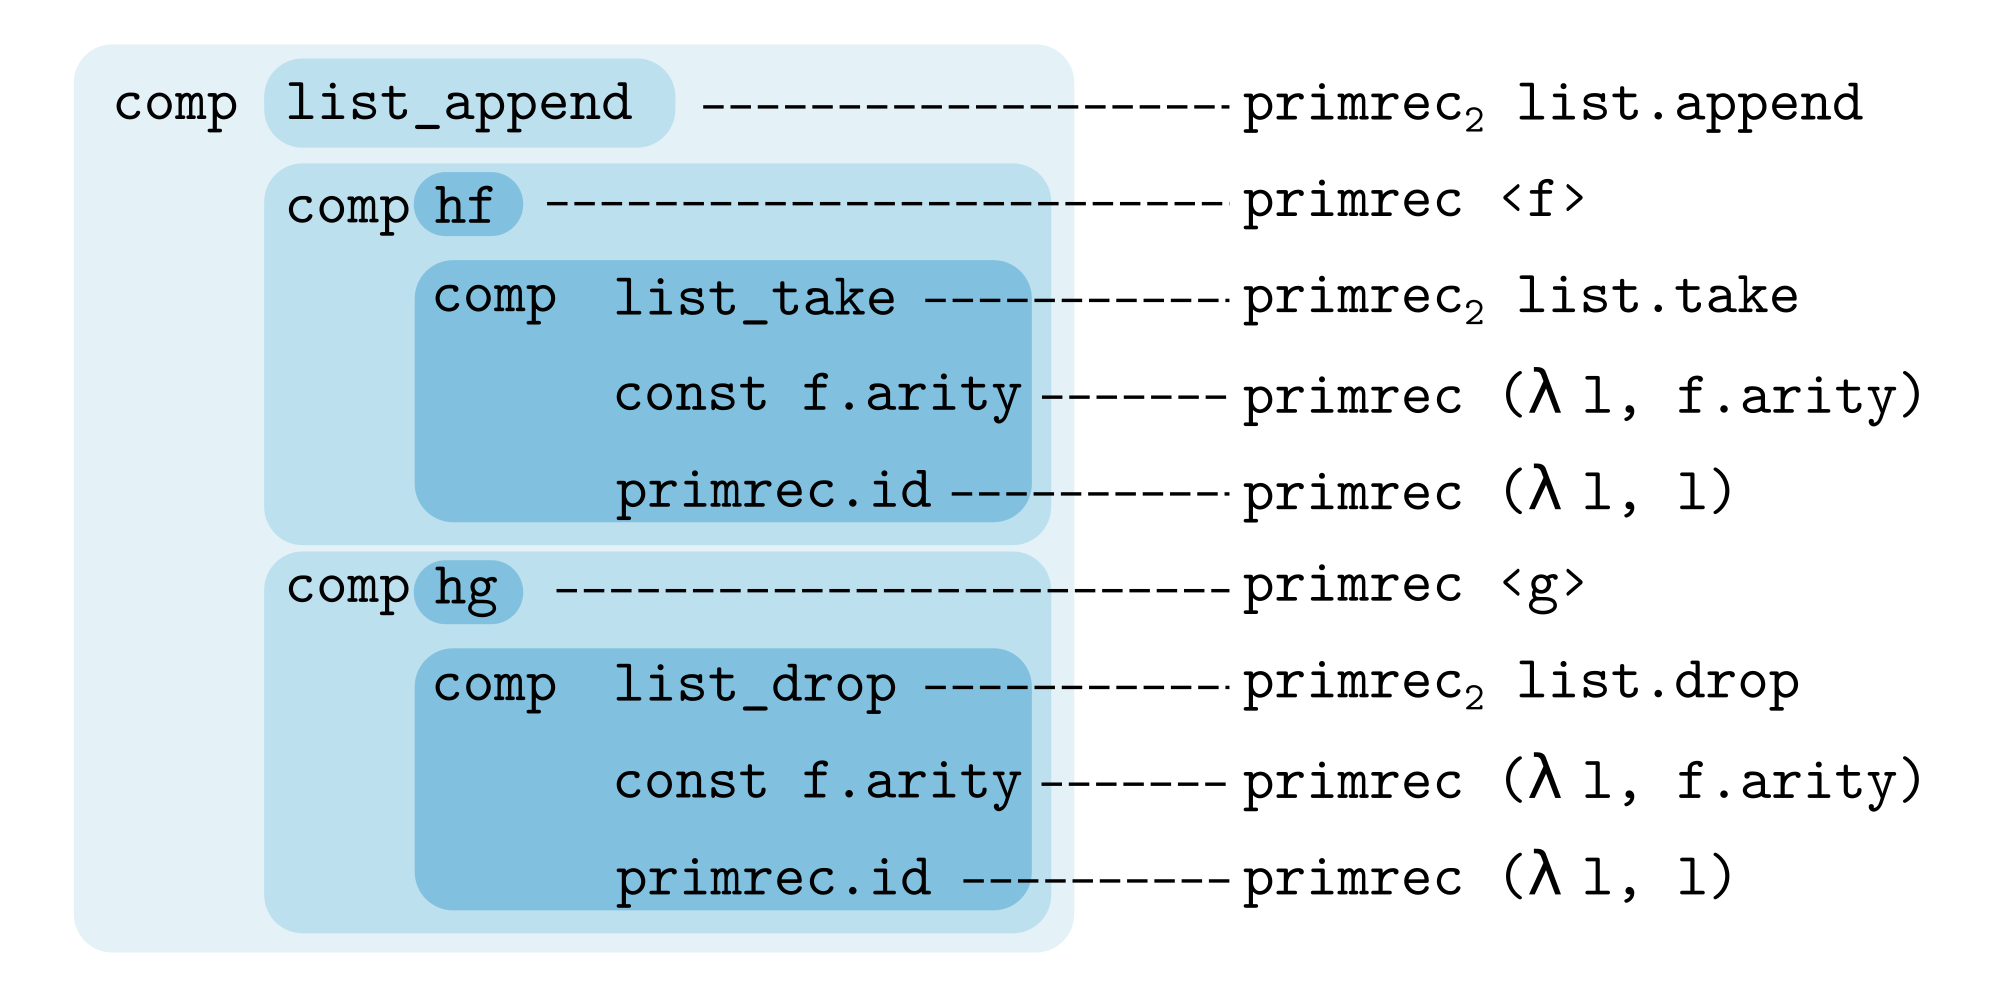
\includegraphics[width=0.9\textwidth]{drawing.png}
    \caption{Diagram representing \lstinline|rpp_pa|. For example, the first "\lstinline|comp|" block means that, given the fact that \lstinline|list.take| is \lstinline|primrec₂| and \lstinline|(λ l, f.arity)|, \lstinline|(λ l, l)| are \lstinline|primrec|, then the composition \lstinline|list.take f.arity l| is \lstinline|primrec|.}
    \label{fig:rpp_pa}
\end{figure}

We are eventually left with point~\ref{enumerate: drop primrec} of the proof of \lstinline|lemma rpp_pa|, i.e.\@ the proofs of \lstinline|lemma list_take|, and \lstinline|lemma list_drop|.

\vspace{\baselineskip}
\noindent
Let us start by focusing on:
\begin{lstlisting}
        lemma list_take : primrec₂ list.take
\end{lstlisting}
\noindent
in which, we recall, \lstinline|list.take| is defined as:
\begin{lstlisting}
        def take : ℕ → list α → list α
        | 0        a        := []
        | (succ n) []       := []
        | (succ n) (x :: r) := x :: take n r
\end{lstlisting}
\noindent
i.e.\@ a function recursive in both its arguments. The built-in \LEAN recursion principles for \lstinline|ℕ|, and \lstinline|list α| are both proven to be \lstinline|primrec| in \MATHLIB through theorems \lstinline|nat_elim| and \lstinline|list_rec|; unfortunately we cannot use them simultaneously for free in order to reason by induction on \lstinline|take|.

\vspace{\baselineskip}
\noindent
We overcome the problem in two steps:
\begin{enumerate}
    \item we define an ``auxiliary'' function \lstinline|take2| in terms of the known function \lstinline|foldl|, already proven to be \lstinline|primrec|, and prove that \lstinline|take2| is \lstinline|primrec|;
    \item we prove that \lstinline|take2| is equal to \lstinline|take| for all inputs, and conclude using \lstinline|of_eq|.
\end{enumerate}
The proof of equivalence is established through the use of the ``special'' induction principle \lstinline|list.reverse_rec_on| which decomposes a list into its final element and all preceding elements, rather than the head and tail, feature that helps to reason with \lstinline|take2|'s definition.

\vspace{\baselineskip}
\noindent
Once proven \lstinline|list_take|, we can focus on the proof of \lstinline|list_drop|.
The key step is \lstinline|lemma reverse_drop| here below:
\begin{lstlisting}
    lemma reverse_drop {α : Type*} (n : ℕ) (l : list α) :
        (l.drop n) = reverse (l.reverse.take (l.length - n))
\end{lstlisting}
\noindent
Clearly, it expresses \lstinline|list.drop| in terms of \lstinline|list.take|, so the proof that \lstinline|list.drop| is \lstinline|primrec| proceeds smoothly and this concludes our overview of how the proof of \lstinline|lemma rpp_pa| works.

\vspace{\baselineskip}
Proving that \lstinline|Co|, \lstinline|It|, and \lstinline|If| are \lstinline|primrec| gets simpler to handle because the relevant functions are already proven to be \lstinline|primrec|.

%%%%%%%
\subsection{Base cases}
The base cases are handled in a similar way, by building each function from simpler ones. In particular, the operations \lstinline|Ne|, \lstinline|Su|, \lstinline|Pr| which respectively represent negation $x\mapsto-x$, successor $x\mapsto x+1$, predecessor $x\mapsto x-1$, all represent functions of type \lstinline|ℤ → ℤ|. Instead of focusing specifically on those functions, we found that it was actually easier to start from more basic functions close to the definition of integers in \LEAN, and progressively build more complex functions following exactly their definition and development in the \MATHLIB library. We now focus on those more basic functions.

\vspace{\baselineskip}
Let us look at the definition of integers:
\begin{lstlisting}
    inductive ℤ : Type
    | of_nat : ℕ → ℤ
    | neg_succ_of_nat : ℕ → ℤ
\end{lstlisting}
\noindent
It is based on the two functions/constructors \lstinline|of_nat|, and \lstinline|neg_succ_of_nat| which can be proven to be \lstinline|primrec| almost directly by unfolding the definitions of the embedding \lstinline|ℤ → ℕ| and noticing that through the compositions, the functions become two known functions \lstinline|nat_bit0, nat_bit1 : ℕ → ℕ| which are already proven to be \lstinline|primrec| in \MATHLIB.

Other than \lstinline|of_nat| and \lstinline|neg_succ_of_nat|, the last important building block for functions of type \lstinline|ℤ → ℤ| is the ``Cases Principle'' \lstinline|int.cases_on| for integers:
\begin{lstlisting}
int.cases_on : Π {f:ℤ → Type} (z:ℤ),
    (Π (n:ℕ), f (int.of_nat n)) →
    (Π (n:ℕ), f (int.neg_succ_of_nat n)) → f z
\end{lstlisting}
\noindent
It states that if a function is defined for natural numbers and for negative numbers, then it is defined for all numbers.
The reason this is important is that almost all basic functions with domain \lstinline|ℤ| are defined by cases, breaking down the case where the input number is natural and where it is negative. We can express the fact that this cases principle is \lstinline|primrec| in the following way:\footnote{The statement was slightly modified for simplicity. The original statement can be found in \cite{MalettoRPPLEAN2021}.}
\begin{lstlisting}
    lemma int_cases {f:α → ℤ} {g h:α → ℕ → β}
        (hf : primrec f) (hg : primrec₂ g) (hh : primrec₂ h) :
        primrec (λ a, int.cases_on (f a) (g a) (h a))
\end{lstlisting}
\noindent
This means that given three \lstinline|primrec|/\lstinline|primrec₂| functions \lstinline|hf, hg, hh|, we can compose them with the ``Cases Principle'' to get a new function, which the lemma states is \lstinline|primrec|.
We remark that all other cases/recursion/induction principles in \MATHLIB are stated in a similar fashion. The proof, as usual, is based on the fact that more elementary operations are already proven to be \lstinline|primrec| in \MATHLIB.

%=====================
\section{Conclusion and developments}
\label{section:Conclusion and developments}
We give a concrete example of reversible programming in a proof-assistant. We think it is a valuable operation because programming reversible algorithms is not as much wide-spread as classical iterative/recursive programming, in particular by means of a tool that allows us to certify the result.
Other proof assistants have been considered, and in fact the same theorems have also been proved in \COQ, but we found that the use of the \MATHLIB library together with the \lstinline|simp| tactic made our experience with \LEAN much smoother.
Furthermore, our work can migrate to \LEANFour whose stable release is announced in the near future. \LEANFour exports its source code as efficient \CPP code \cite{2021-LEAN4-MouraUllrich}; our and other reversible algorithms can become efficient extensions of \LEANFour, or standalone.

The most application-oriented obvious goal to mention is to keep developing a Reversible Computa\-tion-centered certified software stack, spanning from a programming formalism more friendly than \lstinline|rpp|, down to a certified emulator of \PISA, passing through compilator, and optimizer whose properties we can certify. For example, we can also think of endowing \PISA emulators with energy-consumption models linked to the entropy that characterize the reversible algorithms we program, or the \PISA object code we can generate from them.

A more speculative direction, is to keep exploring the existence of programming schemes in \lstinline|rpp| able to generate functions, other than Cantor Pairing, etc., which we can see as discrete space-filling functions, whose behavior we can describe as steps, which we count, along a path in some space.

%------------------
\bibliographystyle{elsarticle-num}
\bibliography{bib-minimal}

%\appendix

\end{document}